\documentclass[10pt,fleqn]{article}

\usepackage[english]{babel}
\usepackage[utf8x]{inputenc}
\usepackage{enumerate}
\usepackage{amsmath}
\usepackage{amssymb}
\usepackage{amsfonts} 
\usepackage{mathtools}
\usepackage{graphicx}
\usepackage{bm}
\usepackage[usenames,dvipsnames]{color}
\usepackage{todonotes}
\usepackage{dsfont}
\usepackage{hyperref}
\hypersetup{
    colorlinks,
    citecolor=black,
    filecolor=black,
    linkcolor=black,
    urlcolor=black
}
\usepackage{algorithm}
\usepackage{algorithmic}
\usepackage{appendix}
\usepackage{subcaption}
\usepackage{fancyvrb}
\usepackage{subfigure}
\usepackage{graphicx,xcolor}
\usepackage{pifont,mdframed}
\usepackage{tikz}
\usepackage{bm}
\usetikzlibrary{fit,positioning}


%
% Macros
%
\newcommand \cashort[1] { {\todo[color=yello]{#1 -- Cedric}} }
\newcommand \calong[1]  { { \todo[inline,color=yellow]{#1 -- Cedric} } }
\newcommand \gbshort[1] { {\todo[color=cyan!40]{#1 -- Guillaume}} }
\newcommand \gblong[1]  { { \todo[inline, color=cyan!40]{#1 -- Guillaume} } }
\newcommand \mgshort[1] { {\todo{#1 -- Mark}} }
\newcommand \mglong[1]  { { \todo[inline]{#1 -- Mark} } }
\newcommand \bfshort[1] { {\todo[color=green!40]{#1 -- Bryan}} }
\newcommand \bflong[1]  { { \todo[inline,color=green!40]{#1 -- Bryan} } }


% Adds a plus const to the end of a math expression
\def \pcst{+\text{const}}

% A fancy version for capital R
\def \Rcal{\mathcal{R}}

% A fancy version for r
\def \rcal{\mathbf{r}}

% Loss function / log likelihood as appropriate
\def \L{\mathcal{L}}

% KL divergence [Math Mode]
\newcommand{\kl}[2] {
	\text{KL}\left[#1||#2\right]
}

\newcommand \vecf[1] {
    \text{vec}\left(#1\right)
}

\newcommand \ent[1] {
    \text{H} \left[ #1 \right]
}

\newcommand \mut[2] {
    \text{I} \left[ #1 ; #2 \right]
}

\newcommand \dvi[2] {
    \text{D}_\text{VI} \left[ #1; #2 \right]
}

% Starts an expected value expresses [Math Mode]
\newcommand{\starte}[1] {%
	\mathbb{E}_{#1}\left[
}

% Ends an expected value expression [Math Mode]
\def \ende{\right]}

% Starts an varianc expresses [Math Mode]
\newcommand{\startv}[1] {%
	\mathbb{V}\text{ar}_{#1}\left[
}

% Ends an variance expression [Math Mode]
\def \endv{\right]}

%\newcommand \ex[2] {
%    \bigl\langle #1 \bigr\rangle_{#2}
%}
\newcommand \ex[2] {
    \mathbb{E}_{ { #2 } }\left[ #1 \right]
}
\newcommand \var[2] {
    \mathbb{V}ar_{ { #2 } }\left[ #1 \right]
}

\newcommand \halve[1] {
	\frac{#1}{2}
}

\newcommand \half {
    \halve{1}
}

\newcommand \tr { \text{tr} } 

\newcommand \T { ^\top } 

\newcommand \fixme[1] {
    {\color{red} FIXME: #1}
}

\newcommand \vv[1] { \bm #1 }

\newcommand{\mbeq}{\overset{!}{=}}

\newcommand \diag[1] { \text{diag} \left( {#1} \right) }
\newcommand \diagonal[1] { \text{diagonal} \left( {#1} \right) }

\newcommand \Ed {{ \vv{\xi}_d}}
\newcommand \Edj {{\xi_{dj}}}
\newcommand \Edk {{\xi_{dk}}}
\newcommand \AEdj {{\Lambda(\xi_{dj})}}
\newcommand \AEdk {{\Lambda(\xi_{dk})}}
\newcommand \AEd  {{ \bm{\Lambda}(\bm{\xi}_d) }}

\newcommand \Axi { { \Lambda_{\xi} } }
\newcommand \bxi { { \vv{b}_{\xi} } }
\newcommand \cxi { { c_{\xi} } }


\newcommand \wdoc      { { \vv{w}_d } }
\newcommand \wdt[0]  { { w_{dt} } }
\newcommand \wdn[0]  { { \vv{w}_{dn} } }
\newcommand \wdnt[0]  { { w_{dnt} } }
\newcommand \wdd[0]   { { \vv w_{d} } }
\newcommand \zd[0]   { { \vv z_{d} } }
\newcommand \zdn[0]  { { \vv{z}_{dn} } }
\newcommand \zdnk[0] { { z_{dnk} } }
\newcommand \zdk[0]  { { z_{dk} } }
\newcommand \thd[0]  { { \vv \theta_d } }
\newcommand \thdk[0] { { \theta_{dk} } }
\newcommand \thdj[0] { { \theta_{dj} } }
\newcommand \epow[1] { { e^{#1} } }
\newcommand \pkt     { { \phi_{kt}  } }
\newcommand \pk      { { \vv \phi_k } }
\newcommand \lmd     { { \vv \lambda_d } }
\newcommand \lmdk    { { \lambda_{dk} } }
\newcommand \xd      { { \vv x_d } }
\newcommand \atxd     { A ^\top \bm x_d}
\newcommand \axd     { A\bm x_d}
\newcommand \tsq      { { \tau^2 } }
\newcommand \ssq      { { \sigma^2 } }
\newcommand \tmsq     { { \tau^{-2} } }
\newcommand \asq      { { \alpha^2 } }
\newcommand \amsq     { { \alpha^{-2} } }
\newcommand \sgsq     { { \sigma^2 } }
\newcommand \xvec     { { \vv{x} } }
\newcommand \omk      { { \bm \omega _k } }
\newcommand \omkt     { { \omega_{kt} } }
\newcommand \oma     { { \Omega_A } }
\newcommand \gdn      { { \vv{\gamma}_{dn} } }
\newcommand \gdnk     { { \gamma_{dnk} } }
\newcommand \gdk      { { \gamma_{dk} } }
\newcommand \isigt   { { \Sigma^{-1}_{\bm \theta} } }




\newcommand \halfSig { \frac{1}{2\sigma^2} }

\newcommand \nor[2]   { \mathcal{N} \left( {#1}, {#2} \right) }
\newcommand \nord[3]   { \mathcal{N}_{#1} \left( {#2}, {#3} \right) }
\newcommand \mnor[3]  { \mathcal{N} \left(#1, #2, #3\right) }
\newcommand \norp[3]  { \mathcal{N} \left(#1; #2, #3\right) }
\newcommand \mnorp[4] { \mathcal{N} \left(#1; #2, #3, #4\right) }
\newcommand \mul[1]   { \mathcal{M} \left( {#1} \right) }
\newcommand \muln[2]  { \mathcal{M} \left( {#1},{#2} \right) }
\newcommand \dir[1]   { \mathcal{D} \left( {#1} \right) }
\newcommand \pois[1]  { \mathcal{P} \left( {#1} \right) }
\newcommand \gp[2]    { \mathcal{GP} \left( {#1}, #2 \right) }
\newcommand \dir[1]   { \mathcal{D} \left( {#1} \right) }
\newcommand \gam[2]   { \mathcal{G} \left( {#1}, {#2} \right) }
\newcommand \beta[1]  { \mathcal{B}eta \left( {#1}, {#2} \right) }

\newcommand \lne[1]  { { \ln \left( 1 + e^{ #1 } \right) } }
\newcommand \Tr[1]   { \tr \left(  {#1}  \right) }

\newcommand \roud  { \vv{\rho}_{d}  }
\newcommand \rodk { \rho_{dk} }

\newcommand \exA[1]  { \ex{#1}{q(A)} }
\newcommand \exV[1]  { \ex{#1}{q(V)} }
\newcommand \exT[1]  { \ex{#1}{q(\Theta)} }
\newcommand \extd[1] { \ex{#1}{q(\thd)} }
\newcommand \exTV[1] { \ex{#1}{q(\Theta)q(V)} }

\newcommand \Real[0]  { { \mathbb{R} } }
\newcommand \VReal[1] { { \mathbb{R}^{#1} } }
\newcommand \MReal[2] { { \mathbb{R}^{#1 \times #2} } }
\newcommand \Nat[0]  { { \mathbb{N} } }
\newcommand \VNat[1] { { \mathbb{N}^{#1} } }
\newcommand \MNat[2] { { \mathbb{N}^{#1 \times #2} } }

\newcommand \inv[1] { {#1}^{-1} }
\newcommand \invb[1] { \inv{\left( #1 \right)} }

\newcommand \cn { \textsuperscript{\texttt{[{\color{blue}Citation Needed}]}} }

\newcommand \const { { \text{c} } }

\providecommand \floor [1] { \left \lfloor #1 \right \rfloor }
\providecommand \ceil [1] { \left \lceil #1 \right \rceil }


\newcommand \vt[2] { { #1^{(#2)} } }

\newcommand \hashtag[1] { { \ttfamily \##1 } }

\newcommand \mvy  { \vv{m}_{\vv{y}} }
\newcommand \sigvy { { S_Y } }

\newcommand \mmy  { M_Y      }
\newcommand \md   { \vv{m}_d }
\newcommand \phin { \vv{\phi}_n }
\newcommand \isigma { { \inv{\Sigma} } }

\newcommand \sigv     { { \Sigma_V } }
\newcommand \isigv     { { \Sigma^{-1}_V } }

\newcommand \sigy { { \Sigma_Y } }
\newcommand \isigy { { \Sigma_{-1}_Y } }


\newcommand \omy  { { \Omega_Y } }
\newcommand \iomy { { \inv{\Omega_Y} } }

\newcommand \siga     { { \Sigma_A } }
\newcommand \isiga     { { \Sigma^{-1}_A } }
\newcommand \diagv { { \diag{\nu_1,\ldots,\nu_P} } }

\newcommand \ma { \vv{m}_a }
\newcommand \my { \vv{m}_y }

\newcommand \VoU { V \otimes U }

\newcommand \one { \mathbb{1} }
%\newcommand \one  {{  \mathds{1} }}

\newcommand \lse { \text{lse} }
%\newcommand \lse[0] { \mathrm{lse} }

% Conditional independence 
\def\ci{\perp\!\!\!\perp} % from Wikipedia



% ------ For the eval section

% Multinomial PDF [Math Mode]
% params: 1 - the variable
%         2 - the value
%         3 - the state indicator (e.g. k for a distro with K values)
%         4 - any additional subscript
\newcommand{\mpdf}[4] {
	\prod_{#3} {#1}_{{#4} {#3}} ^ {#2}
}

% Dirichlet PDF [Math Mode]
% params: 1 - the variable
%         2 - the hyper-parameter
%         3 - the state indicator (e.g. k for a distro with K values)
%         4 - any additional subscript
\newcommand{\dpdf}[4] {
	\frac{1}{B({#2})} \prod_{#3} {#1}_{{#4} {#3}} ^ {({#2}_{#3} - 1)}
}

% To simplify the sampling equations, this is indicates
% that the given value has had datapoint "m" stripped out
%
\newcommand{\lm}[1] {
	#1^{\setminus m}
}

\newcommand \model[0] {
    \mathcal{M}
}

\newcommand \perplexity[1] {
    \mathcal{P} \left( { #1 } \right)
}

\newcommand \WTrain {
    \mathcal{W}^{(t)}
}

\newcommand \WQuery {
    \mathcal{W}^{(q)}
}

\newcommand \oneover[1] {
    \frac{1}{ {#1} }
}

\newcommand \samp[1] {
    { #1 }^{(s)}
}

\newcommand \etd[0] {
    \vv{\eta}_d
}

\begin{document}



\newcommand \xdn  { { \vv{x}_{dn} } }
\newcommand \zd   { { \vv{z}_d } }
\newcommand \qfam { { \mathcal{Q} } }
\newcommand \xdat { { \mathcal{X} } }
\newcommand \zdat { { \mathcal{Z} } }
\newcommand \xnew { { \vv{x}^{*} } }
\newcommand \znew { { \vv{z}^{*} } }
\newcommand \param { { \vv{\phi} } }
\newcommand \params { { \Phi } }
\newcommand \ml[1] { { {#1}_{\text{ML}} } } 
\newcommand \map[1] { { {#1}_{\text{MAP}} } } 
\newcommand \quarter { { \oneover{4} } }
\newcommand \eighth { { \oneover{8} } }
\newcommand \fqt[1] { { \mathcal{F}\left( {#1} \right) } }
\newcommand \joint { { p(\xdat, \zdat | \params) } }
\newcommand \logjoint { { \ln \joint } }
\newcommand \exlogjoint[1] { { \ex{\logjoint}{{#1}} } }

\chapter{Probabilistic Inference with Text}
This chapter reviews of probabilisitic inference from a Bayesian perspective. We introduce maximum-likelihood, maximum-a-posteriori, and fully Bayesian Inference. We describing inference schemes for latent variable models, and extend this to inference on large datasets using stochastic gradient descent (SGD), natural gradients, and biased sampling schemes. Finally, we provide a brief overview on Bayesian non-parametrics, and discuss the problem of evaluating model-fit.

Throughout, we use inference on text as a motivating example, and introduce language models, mixture-models of text, and admixture models of text, the last known colloquially as ``topic models". We quantitatively evaluate the effect that choices in models and inference schemes may have, and demonstrate the effect of different choices of evaluation metric.
\section{Inference Methods}

Probabilistic inference is concerned with two problems: inference, the estimation of parameter values $\param$ from a set of observations $\vv{x} \in \xdat$; and prediction, the evaluation of the probability of unobserved variables $p(\xnew | \xdat) = \int p(\xnew | \param) p(\param | \xdat) d\param$. Various methods have been proposed for this purpose.


\emph{Maximum likelihood} finds the parameter value that maximises, $p(\xdat|\param)$, known as the likelihood. For reasons of algebraic convenience\footnote{The log-likelihood can also be motivated by Information Theory. Since mean negative log-likelihood asymptotically converges to the Shannon-Entropy, minimising it leads to a model that better ``compresses" data. This idea is discussed in detail in \cite{MacKay2005InfoTheory} }, one commonly finds the maximum of the log of the likelihood.

% For MLE / Info Theory: https://quantivity.wordpress.com/2011/05/23/why-minimize-negative-log-likelihood/
% http://thirdorderscientist.org/homoclinic-orbit/2013/4/1/maximum-likelihood-and-entropy
\begin{align}
\ml{\param} = \arg \max_{\param} \ln p(\xdat | \param)
\end{align}

As the log of a monotonically increasing function, the log-likelihood and likelihood have the same maxima. For the particular case of independently and identically distributed (IID) observations, the log-likelihood factors into a simple sum.

\begin{align}
\ml{\param} = \arg \max_{\param} \sum_d \ln p(\xd | \param) \label{eqn:log-like-iid-decomp}
\end{align}


For prediction one typically employs the approximation

\begin{align}
p(\xnew | \xdat) 
&= \int p(\xnew | \param) p(\param | \xdat) d\param \label{eqn:ml-prediction}\\
&\approx \int p(\xnew | \ml{\param}) p(\param | \xdat) d\param
=  p(\xnew | \ml{\param})
\end{align}

The same decomposition used in \eqref{eqn:log-like-iid-decomp} can also be derived from the assumption that the data are \emph{exchangeable}.  A finite sequence of random variables $\xdat = \{\xd\}_{d=1}^{D}$ is exchangeable if its joint distribution is invariant to any permutation of its order. An infinite sequence is exchangeable, if all finite subsequences are themselves exchangeable. The link with IID observations is provided by DeFinetti's theorem (extended to the multinomial case\bfshort{What is the ``multinomial case"} in \cite{Hewitt1955}) which states that the joint distribution of an exchangeable sequence of variables is equivalent to sampling a random parameter $\param$ from some prior distribution, then sampling IID random variables conditional on that random parameter such that $p\left(\xdat\right) = \prod_d p(\xd | \param)$.

\emph{Maximum a Posteriori} (MAP) estimation, like maximum likelihood, finds a mode, but of the posterior distribution instead of the likelihood. Given a prior $p(\param)$, the posterior is given by Bayes rule:
\begin{align}
p(\param | \xdat) = \frac{p(\xdat | \param)p(\param)}{p(\xdat)} = \frac{\text{likelihood} \times \text{prior}}{\text{evidence}}
\end{align}

The MAP solution is:

\begin{align}
\map{\param} = \arg \max_{\param} \frac{p(\xdat | \param)p(\param)}{p(\xdat)}
 & = \arg \max_{\param} p(\xdat | \param)p(\param) \\
 & = \arg \max_\param \ln p(\xdat | \param) + \ln p(\param)
\end{align}
Prediction follows similarly to ML
\begin{align}
p(\xnew | \xdat) \approx \int p(\xnew | \map{\param})p(\param|\xdat)d\param = p(\xnew | \map{\param})
\end{align}



The incorporation of the prior is motivated by two related reasons: firstly it allows a practitioner to supply some prior knowledge to the inference procedure and secondly it prevents a model from overfitting in the presence of limited or noisy data.

The alternative to finding modes is to take a fully \emph{Bayesian} approach, solve Bayes rule directly, and thereby derive a \emph{distribution} over $\param$. This in turn means we can evaluate our predictions exactly, by solving the integral \eqref{eqn:ml-prediction} and thereby get a measure of the uncertainty in our predictions.

The Bayesian approach involves evaluating the evidence $p(\xdat) = \int p(\xdat | \param) p(\param) d\param$. In many cases this is intractable, but there are families of prior and likelihood distributions where the prior and posterior have the same functional form for which exact inference is possible. In these cases we say the prior is \emph{conjugate} to the likelihood.

An example is learning a parameter $\param$ with a Dirichlet distribution given multinomial-distributed observations (e.g. throws of a weighted dice). The Dirichlet distribution is given by:
\begin{align}
p(\param) & = \oneover{B(\vv{\beta})} \prod_k \phi_k^{(\beta_k - 1)} &
B(\vv{\beta}) & = \frac{\prod_k \Gamma(\beta_k)}{\Gamma(\sum_k \beta_k)}
\end{align}
where $B(\cdot)$ is the multivariate beta function, and $\Gamma(\beta)$ is the Gamma function, which can be thought of as a continuous generalisation of the factorial function such that $x! = \Gamma(x+1)$. The multinomial is given by:
\begin{align}
p(\vv{x}|\param) = \frac{(\sum_k x_k)!}{\prod_k x_k!} \prod_k \phi_k^{x_k}
\end{align}
though for a single draw, the  quotient evaluates to one. A single-draw multinomial distribution is known as a \emph{categorical} distribution, and will be denoted in this thesis with the notation $\vv{x}|\param \sim \cat{\param}$. The joint distribution of several, exchangeable observations using a categorical likelihood is 
\begin{align}
p(\xdat|\param) & = \prod_d \prod_k \phi_k^{x_{dk}} = \prod_k \phi_k^{n_k} &
n_k = \sum_d x_{dk}
\end{align}
Using this we can analytically evaluate the evidence $p(\xdat)$:
\begin{align}
p(\xdat) & = \frac{1}{B(\beta)} \int \prod_k \phi_k^{n_k} \prod_k \phi_k^{(\beta_k - 1)} d\param  = \frac{1}{B(\beta)} \int \prod_k \phi_k^{n_k + \beta_k - 1} \\
& = \frac{B(\vv{n} + \vv{\beta})}{B(\vv{\beta})} \label{eqn:polya-is-evidence}
\end{align}
The analytic solution arises from observing that the integrand is an unnormalised Dirichlet distribution parameterised by $\vv{n} + \vv{\beta}$ where $\vv{n} = \{ n_k \}_{k=1}^K$. This marginal distribution is sometimes known as the P\'{o}lya distribution, or the Dirichlet-compound-Multinomial distribution \cite{Madsen2005}.\label{polya}

Putting this together we can analytically derive an expression for the posterior:

\begin{align}
\begin{split}
p(\phi|\xdat) 
& = \frac{p(\phi|\xdat)p(\phi)}{p(\xdat)}
 = \left(\prod_k \phi_k^{n_k} \right)
   \left(\oneover{B(\vv{\beta})} \prod_k \phi_k^{\beta_k - 1} \right)
   \frac{B(\vv{\beta})}{B(\vv{n} + \vv{\beta})} \\
& = \oneover{B(\vv{n} + \vv{\beta})} \prod_k \phi_k^{n_k + \beta_k - 1}
\end{split}
\end{align}
which is a Dirichlet distribution parameterised by $\vv{n} + \vv{\beta}$

It is useful to compare the expected value of the posterior with the MAP and maximum likelihood solutions.

\begin{align}
\ex{\phi_k}{}  &= \frac{n_k + \beta_k}{\sum_j n_j + \beta_j} &
\phi_k^{\text{MAP}} &= \frac{n_k + \beta_k - 1}{\sum_j n_j + \beta_j - 1} &
\phi_k^{\text{ML}}  &= \frac{n_k}{\sum_j n_j}
\end{align}

The Bayesian approach is more affected by the prior than the MAP solution, where the prior is discounted, and the ML approach obviously incorporates no prior information whatsoever. 

\subsubsection*{A Note on Categorical and Multinomial Distributions}
In this thesis, we will frequently posit models where we sample words one at a time. 

One representation is to use a scalar $x \in \{1 \ldots T\}$ whose value indicates the word chosen. This gives rise to a \emph{categorical} distribution parameterised by a vector $\vv{\phi} \in \VReal{T}$
\begin{align}
x &\sim \cat{\vv{\phi})}&
p(x) = \prod_t \phi_t^{[x = i]}
\end{align}
where $[x = i]$ is the Iverson bracket -- an extension of the Dirac delta -- which evaluates to 1 if the condition is true, and zero otherwise. 

An equivalent representation is a 1-of-T vector $\vv{x}$, where all elements are set to zero except one which is set to 1, one whose index indicates the word chosen. This gives rise to a multinomial distribution parameterised by a vector $\vv{\phi} \in \VReal{T}$ for which the number of trials is fixed at 1.
\begin{align}
\vv{x} &\sim \muln{\vv{\phi}}{1} &
p(x) = \frac{1!}{\prod_t x_t!}\prod_t \phi_t^{x_t} = \prod_t \phi_t^{x_t}
\end{align}
In all cases in this thesis, when we say a variable has a \emph{categorical distribution}, we mean to say it is a 1-of-T vector with a multinomial distribution for which the number of trials is fixed at one. 

 
\subsection*{Example: Language Models}
 \label{sec:langmodels}
An example of conjugate inference is the language-modelling problem. This is the problem of predicting the next word in a sequence of discrete observations from a finite vocabulary (e.g a sentence) given all previous observations. Common use-cases are predictive keyboards, spell-checkers and speech recognition.\bfshort{Cite use-cases}

As vocabularies are normally quite large (typically of the order of 30,000 terms), raising this to the power of two or three can lead to models that are over-parameterised: in particular maximum likelihood estimates will often collapse to zero in the absence of training data. ``Laplace smoothing", equivalent to MAP inference using a symmetric Dirichlet prior, is a simple remedy, but unsatisfying in that it does not take into account the information available in the lower-order n-grams.

Using conjugate Bayesian inference it is possible to create a first-order (i.e. bigram) language model\cite{MacKay1995} that uses unigram statistics. Given a sequence of observations $x_1, \ldots, x_D$, where each $x_d \in \{1 \ldots T\}$, we can define for each of the $T$ words a distribution over the next possible word $\vv{\phi}_t \in \VReal{T}$.

\begin{align}
x_i | x_{i - 1} 
& \sim \cat{\vv{\phi}_{x_{i-1}}}
& \vv{\phi}_t 
& \sim \dir{\vv{\beta}}
\end{align}

As before, used a corpus W to estimate our parameters, the \emph{exact} predictive distribution is
\begin{align}
p(w_i = t | w_{i-1}, W)
& = \ex{\phi_{w_{i-1},t}}{}
  = \frac{n_{w_{i-1},t} + \beta_t}{\sum_v n_{w_{i-1},v} + \beta_v}
\end{align}
where $n_{w_{i-1},t}$ denotes the number of times value $t$ was observed immediately after the value of $w_{i-1}$. The preceding sequence (in this case a single term) is known as the \emph{context}

Since the prior term $\beta_v$ will occur in all contexts, one can incorporate unigram probabilities in our bigram estimates by learning the prior $\vv{\beta}$. This approach, of sharing information between contexts in an inference task, is sometimes known as \emph{multi-task learning} and will be discussed in detail in Chapter 3.

Marginalising out the parameters $\vv{\phi}_t$ provides the model evidence $p(W|\vv{\beta})$ as in equation \eqref{eqn:polya-is-evidence}. The derivative of this with respect to $\beta_v$ is:
\begin{align}
\frac{d \ln p(W|\vv{\beta})}{d\beta_v} =
\sum_t
     \Psi(\sum_u \beta_u) 
     - \Psi(n_{\cdot|t} + \sum_u \beta_u)
     + \Psi(n_{v|t} + \beta_v)
     - \Psi(\beta_v)
\end{align}
where $n_{v|t}$ is the number of times word $v$ has been seen after word $t$ and $n_{\cdot|t} = \sum_v n_{v|t}$. The digamma function $\Psi(\cdot)$ is the derivative of the gamma function $\Gamma(\cdot)$. This leads to a simple re-estimation method for $\beta_v$

\begin{align}
\beta^{new}_v = \beta_v \frac{
        \sum_t \Psi(n_{v|t} + \beta_v) - \Psi(\beta_v)
    }{
        \sum_t \Psi(n_{\cdot|t} + \sum_u \beta_u) - \Psi(\sum_u \beta_u)
    }
\end{align}


There are in fact a variety of methods of inferring a Dirichlet distribution, which are explored more fully in \cite{Minka2000}. For example, taking the fully Bayesian perspective, one might want to regulate inference over $\vv{\beta}$ by putting priors on it in turn. In this case it's useful to reformulate the Dirichlet as being parameterised by a concentration parameter $\beta$ with a Gamma prior and a base measure $\vv{u}$ on the simplex with a symmetric Dirichlet prior, such that $\vv{\phi}_t  \sim \dir{\beta \cdot \vv{u}}$.


This Bayesian model builds on the frequentist Jelinek Mercer\cite{JelinekMercer1980} interpolated language model, wherein the probability of an n-gram was a weighted combination of the probabilities of all m-grams for $m \in \{n, (n-1), \ldots, 1\}$. In the case of a bigram $p(w_i|w_{i-1}) = \lambda p(w_i|w_{i-1}) + (1 - \lambda) p(w_i)$. Jelinek Mercer required different $\lambda$ for each distinct context (sequence of words $w^i_{i-n+1}$), learned through cross-validation. By contrast, the Baysesian perspective leads to a model that neatly balances between the two based on the number of bigram and unigram observations.

An alternative to interpolation models are ``back-off" language-models. One ``backs off" to a simpler estimate if no data exists to support a higher order estimate, i.e the n-gram count is zero. Back-off models typically use a form of discounting, removing a portion of counts from frequently occurring n-grams and assigning the resultant spare probability mass to lower-order n-grams. The best performing back-off model is Knesser-Ney \cite{Chen1999} , which defines the probability of a word as 
\begin{align}
p_\text{KN}(w_i | w^{i-1}_{i-n+1}) = \left\{ \begin{array}{lr}
     \frac{\max\{c(w^i_{i-n+1}) - D, 0\}}{\sum_{w_i} c(w^i_{i-n+1})} & \text{if } c(w_i, w_{i-1}) > 0 \\
     \lambda(w^{i-1}_{i-n+1}) p_\text{KN}(w_i | w^{i-1}_{i-n+2}) & \text{otherwise}
 \end{array}
\right.
\end{align}
where $c(\cdot)$ denotes how often the word sequence was observed in the data. In order to accumulate enough probability mass to assign to the unobserved n-grams, mass is ``skimmed" off the observed n-grams using the discount term $D$. This is then used in the normalisation term $\lambda(w^{i-1}_{i-n+1}) = \frac{D}{\sum_{w_i} c(w^{i-1}_{i-n+1})}$ which ensures all probabilities sum to 1. The value of $D$ is normally found using cross validation.

One can augment back-off models with interpolation. An interpolated variant of Knesser-Ney called ``modified Knesser-Ney"\cite{Chen1999} is one of the best performing language models currently in use, and performs better than the Bayesian approach described above\cite{Teh2002}. This is defined as

\begin{align}
\begin{split}
p_\text{KN}(w_i | w^{i-1}_{i-n+1}) & = 
\frac{\max\{c(w^i_{i-n+1}) - D, 0\}}{\sum_{w_i} c(w^i_{i-n+1})} \\
& + \lambda(w^{i-1}_{i-n+1}) N_{1+}(w^{i-1}_{i-n+1}, *) p_\text{KN}(w_i | w^{i-1}_{i-n+2})
\end{split}
\end{align}
where $N_{1+}(w^{i}_{i-n}, *)$ is the number of unique contexts (i.e. prefixes) in which the n-gram $w^{i}_{i-n}$ has occurred.  This is a unique feature of interpolated Knesser-Ney: given the sentence ``He left San Francisco via San Francisco airport" a higher unigram probability will be assigned to ``San" as it occurs in two contexts (``left" and ``via") than "Francisco" which only occurs after ``San". Later in this chapter we will introduce a probabilistic alternative to Knesser-Nye when discussing non-parametric Bayesian methods\bfshort{Follow up on this}

A further discussion of language-modeling -- including other interpolation and backoff models such as Katz-Smoothing, Witten-Bell Smoothing, Good-Turing Estimation and Absolute Discounting -- is provided by \cite{Goodman2001}.


 
\section{Latent Variable Models}
Oftentimes it is appropriate to assume that there is some unobserved, latent process which determines the distributions of the observed variables. Denoting the latent variables as $\zdat$ this gives rise to the following likelihood
\begin{align}
p(\xdat|\params) = \int p(\xdat, \zdat|\params) d\zdat
\end{align}

A common case where latent variables arise is the mixture model, where it is assumed there are $K$ distributions, of which one, identified by a latent categorical variable $\vv{z}_d$ is used to sample an observation $\xd$. 

Our MAP solution is
\begin{align}
\begin{split}
\params 
    &= \arg \max_\params \ln p(\params) + \ln p(\xdat|\params) \\
    &= \arg \max_\params \ln p(\params) + \ln \int \joint d\zdat \label{eqn:em-problem}
\end{split}
\end{align}

In this case of a mixture model, since mixture assignments $\vv{z}_d$ have a categorical distribution
\begin{align}
\ln \int \joint d\zdat = \ln \left(\sum_Z \joint\right)
\end{align}

\bfshort{Why does the integral have no analytic solution}
In many cases either the integral in \eqref{eqn:em-problem} has no analytic solution, or evaluating it is simply not tractable. In this case one uses an approximation, leading to the Expectation-Maximisation algorithm.
\subsection{Expectation Maximisation}
Jensen's inequality states that for any \emph{concave} function $f(x)$, $f\left(\ex{x}{}\right) \geq \ex{f(x)}{}$. By introducing an arbitrary distribution $q(\zdat)$ over the latent variables, we can employ the inequality to approximate log-integral in equation \eqref{eqn:em-problem}

\begin{align}
 \ln p(\xdat|\params) & = \ln \int \joint d\zdat =  \ln \int \frac{q(\zdat)}{q(\zdat)} \joint d\zdat\\ 
     &=  \ln \ex{\oneover{q(\zdat)}\joint}{q} \geq  \ex{\ln \oneover{q(\zdat)}\joint}{q}\\
     &= \ex{\ln \joint}{q} + \ent{q} \label{eqn:elbo}
\end{align}
where the entropy $\ent{q} = -\ex{\ln q(\zdat)}{q}$. Equation \eqref{eqn:elbo} is sometimes referred to as the \emph{free energy} or the \emph{evidence lower-bound} (``ELBO").

This leads two a two-step, iterative, maximisation process, where at each iteration $i$ we first find the distribution over our latent variables that maximises the ELBO, and then secondly use that to approximate the integral and find the distribution over our parameters that maximise the likelihood.

\begin{align}
\text{E-Step:} & & q^i(\zdat) & = \arg \max_{q(\zdat)} \ex{\ln p(\xdat, \zdat|\params^{i-1})}{q^{i-1}} + \ent{q} \label{eqn:estep} \\
\text{M-Step:} & & \params^i & = \arg \max_{\params} \ex{\ln \joint}{q^{i}} + \ln p(\params) \label{eqn:mstep}
\end{align}
To determine how to maximise $q(\zdat)$ we observe that, for a fixed $\params$, the difference between the ELBO and the marginal log-likelihood is given by
 the Kullback Leibler divergence between $q(\zdat)$ and the posterior $p(\zdat|\xdat, \params)$.
\begin{align}
\int q(\zdat) \ln \frac{p(\xdat, \zdat|\params)}{q(\zdat)} d\zdat
& = \int q(\zdat) \ln \frac{p(\zdat|\xdat, \params)p(\xdat | \params)}{q(\zdat)} d\zdat \\
& = \int q(\zdat) \ln p(\xdat | \params) q\zdat + \int q(\zdat)\ln\frac{p(\zdat|\xdat, \params)}{q(\zdat)} d\zdat \\
& = \ln p(\xdat | \params) + \kl{q(\zdat)}{p(\zdat|\xdat, \params)}
\end{align}
As the Kullback-Leibler divergence is always positive, reducing the divergence will increase the ELBO. Its maximum, $\ln p(\xdat | \params)$, is attained when $\kl{q(\zdat)}{p(\zdat|\xdat, \params)} = 0$. Therefore the  E-Step maximisation step is to set $q(\zdat) = p(\zdat | \xdat, \param)$.

This is the MAP variant of the Expectation Maximization (EM) algorithm\cite{Dempster1977}. 
Both E and M steps increase the bound. In the M-Step, we maximise the ELBO with respect to $\params$, increasing both the likelihood and the ELBO. In the E-Step by setting $q(\zdat) = p(\xdat|\zdat, \params)$ the KL divergence goes to zero, decreasing the gap between the ELBO and marginal likelihood. Consequently EM is guaranteed to find a local maximum of the marginal likelihood.\bfshort{Reference for convergence}

\subsection*{Example: A Mixture of Multinomials}
\bflong{Add Poisson to Multinomial Here}
As an example, consider the problem of modelling a corpus of documents. Let $\xd \in \mathbb{N}^T$ be the count of how often each word occurred in document $d$, for all $T$ words (known as the bag-of-words model). If we presume each document is about one of K topics, where each topic has a distribution over word-counts $\vv{\phi}_k$, we can associate a latent categorical variable $\vv{z}_d$ with each document indicating which (unobserved) topic generated its words. Denoting document d's word-count as $n_d = \sum_t x_{dt}$, and letting $\params = \{ \vv{\phi}_{k=1}^K \}$, this gives rise to the mixture of multinomials model\cite{Nigam2000}
\begin{align}
\vv{\theta} & \sim \dir{\vv{\alpha}} &
\zd|\vv{\theta} & \sim \cat{\vv{\theta}} & 
\xd|\zd, \params & \sim \prod_k \muln{\param_k}{n_d}^{z_{dk}} & 
\param_k & \sim \dir{\vv{\beta}}
\end{align}
\bflong{Need to note and explain that $\muln{\param_k}{n_d} = \prod_n \cat{\param_k}$}
Note that in this model the Dirichlet hyper-parameters $\vv{\alpha}$ and $\vv{\beta}$ are coupled: small symmetric values of $\vv{\alpha}$ will encode a preference for fewer topics, and therefore require denser vocabularies -- and so larger values of $\vv{\beta}$ -- to generate the observations. 

For brevity we will not consider hyper-parameter inference. 

For a mixture of multinomials model, once we add the constraints that $\sum_k \theta_k = 1$ and $\sum_t \phi_{kt} = 1$, the updates can be derived using the method of partial derivatives with Lagrange multipliers:


\begin{align}
\text{E-Step:} & & q(z_{dk}) 
& = \frac{p(\xd|z_d = k, \param)p(z_d = k)}{\sum_j p(\xd|z_d = j, \param)p(z_d = j)} 
= \frac{p(\xd | \param_k) \theta_k}{\sum_j p(\xd | \param_j) \theta_j} \label{eqn:mom-estep} \\
\text{M-Step:} 
& & \phi_{kt} & =
    \frac{
        \sum_d \ex{z_{dk}}{q}x_{dt} + \beta_t - 1
    }{
        n_k + \sum_v \left( \beta_v - 1 \right)
    } \qquad n_k = \sum_d \ex{z_{dk}}{} \\
& & \theta_k & =  
    \frac{
        n_k + \alpha_k - 1
    }{
        \sum_j n_j + \alpha_j - 1
    } \label{eqn:mom-mstep}
\end{align}
where $\ex{z_{dk}}{q} = q(z_{dk})$. The predictive distribution for a new observation $\xnew$ is:
\bfshort{$\phi_{kt}$ denom looks wrong, it needs normalisation}
\begin{align}
p(\xnew | \xdat, \params)  = \sum_k p(\znew = k | \vv{\theta}) p(\xnew, \znew = k | \param_k) 
\approx \sum_k \theta_k \cdot p(\xnew | \param_k)
\end{align}
where we have approximated the distributions by substituting the MAP estimates for parameter values in our likelihood.

In practical terms, individual word probabilities will be very small, since in even small corpora (e.g. the NIPS dataset\bfshort{reference}) there are usually in excess of 10,000 distinct words. Consequently there is a risk of underflow and catastrophic cancellation when evaluating the likelihood in equation \eqref{eqn:mom-estep}. This is avoided by using log-probabilities wherever possible, leading to the following re-writing of the E-Step above:

\begin{align}
\hat{z}_{dk} = \ln \theta_k + \sum_t w_{dt} \ln \phi_{kt} \\
\ln p(z_{dk} | w_d) = \hat{z}_{dk} - \ln (\sum_j \exp(\hat{z}_{dj})) \label{eqn:mom-lnz-update}
\end{align}
The second term in equation \eqref{eqn:mom-lnz-update} is the log-sum-exp function, which we will discuss in some detail in Chapter 2. In this case, we would like to avoid evaluating the term $\exp(\hat{z}_{dk})$ since that would trigger the underflow problem once more. Fortunately by observing that
\begin{align}
\log(a + b) = \log(a \times (1 + \frac{b}{a})) = \log(a) + \log (1 + \frac{b}{a})
\end{align}
and therefore that
\begin{align}
\ln(e^a + e^b) = \ln (e^a) + \ln (1 + \frac{e^b}{e^a}) = a + \ln(e^{a-a} + e^{b-a})
\end{align}
One can derive the recursive solution
\begin{align}
\ln(\sum_j \exp(\hat{z}_{dj})) = z_{d*} + \ln(\sum_j \hat{z}_{dj})
\end{align}
Where $\hat{z}_{d*} = \arg \max_j \hat{z}_{dj}$

A weakness of mixture-models is that \bfshort{Mixture model problems}



\subsection{Variational EM}
It is not always feasible to evaluate the posterior distribution $p(\zdat|\xdat, \param)$ exactly. In such cases one needs to either approximate the E-Step update to the distribution (e.g. by parameterising it and taking a gradient step\bfshort{Citation}), or approximate the distribution itself.

We consider the latter approach, where one assumes that a good approximation to the true distribution $q(\zdat)$ exists within a family of distributions $\qfam$. One popular choice is the family of factorised distributions $q(\zdat) = \prod_m q(\zdat_m)$. Note that this factorisation is not derived from the IID principle, as the in prior discussion on EM, rather it is a modelling assumption made by the practitioner. The question then is how to evaluate the variational E-Step


\begin{align}
q(\zdat) & = \arg \max_{q(\zdat_1) \ldots q(\zdat_M)} \exlogjoint{\tinymath{\prod_m q(\zdat_m)}} + \ent{q}
\end{align}

Given this formulation, we can solve independently for each block of latent variables $\zdat_m$ in turn, using the following decomposition.

\begin{align}
\begin{split}
& \mathbb{E}_{\tinymath{\prod_m q(\zdat_m)}} \left[ \logjoint \right] + \ent{q} \\
& \qquad = \int q(\zdat_n) \exlogjoint{\tinymath{\prod_{m\neq n} q(\zdat_m)}} d\zdat_n + \ent{q_n} + \sum_{m\neq n} \ent{q_m}
\end{split}\\
\begin{split}
& \qquad = -\kl{q(\zdat_n)}{\tilde{p}(\xdat, \zdat|\param)} + \sum_{m\neq n} \ent{q_m} 
\end{split}
\end{align}

Where $\tilde{p}(\xdat, \zdat|\param)$ is the distribution corresponding to
\begin{align}
\ln \tilde{p}(\xdat, \zdat|\param) = \ex{\logjoint}{\tinymath{\prod_{m\neq n} q(\zdat_m)}} + \text{const}
\end{align}
As the KL divergence is always non-negative, the bound is maximised when it is set to zero, from which the following update is derived: 

\begin{align}
q(\zdat_n) \propto \exp\left( \exlogjoint{\tinymath{\prod_{m\neq n} q(\zdat_m)}}  \right)
\end{align}

Unlike the case of EM however, setting the KL divergence to zero does not cause the ELBO to become equal to the likelihood for a fixed $\params$. This is because the true posterior $p(\zdat | \xdat, \params)$ may not be in the family of distributions $\qfam$ which we have chosen. Consequently, the variational E-Step is not guaranteed to maximise the bound, and so the algorithm is not guaranteed to converge to a local maximum as with EM. Optimising the bound will still improve the likelihood however, and may therefore find useful parameter values. Fuller descriptions of variational learning are given in \cite{Jordan1999a}\cite{Bishop2006}\cite{Tzikas2008}. 

\subsubsection*{Example: Latent Dirichlet Allocation - an Admixture of Multinomials}
An example of variational EM is the latent Dirichlet allocation (LDA) algorithm\cite{BleiNgJordan2003}. Where the mixture of multinomials considered each observation (a document in this example) to be generated by a \emph{single} topic, LDA considers each document to be a generated by a mixture of topics, themselves a subset of the mixture of topics forming the overall corpus, leading to an \emph{admixture} model. 

The inference procedure draws a mixture of topics $\thd$ for a document $d$, then for the each position $n$ in the document, draws a topic $\zdn$ and from it a word $\xdn$
\begin{align}
\thd & \sim \dir{\vv{\alpha}} &
\zdn|\thd & \sim \cat{\thd} & 
\xdn|\zdn, \param & \sim \prod_k \cat{\param_k}^{\zdnk} & 
\param_k & \sim \dir{\vv{\beta}}
\end{align}
Note that whereas $\vv{\theta}$ represented our corpus-level distribution over topics in the mixture of multinomials, $\thd$ now represents our document-level mixture. The corpus-level information is represented by the hyper-parameter $\vv{\alpha}$. 

Letting $\Theta = \{ \thd \}_{d=1}^D$ our MAP algorithm therefore is to evaluate

\begin{align}
\begin{split}
\params 
    &= \arg \max_\params \ln p(\params) + \ln p(\xdat|\params) \\
    &= \arg \max_\params \ln p(\params) + \ln \int \int p(\xdat|\zdat, \Phi)p(\zdat|\Theta) d\zdat d\Theta \label{eqn:vem-lda-problem}
\end{split}
\end{align}

Since it is no longer possible to analytically evaluate the posterior $p(\zdat, \Theta | \xdat)$ we use the variational approximation $p(\zdat, \Theta | \xdat) \approx  q(\zdat)q(\Theta)$. Using this we can derive a lower-bound on the evidence, determine the approximate posteriors and solve for $\params$. Inspection of the ELBO shows the approximation further decomposes as $q(\Theta)q(\zdat) = \prod_d q(\thd)\prod_n q(\zdn)$ from which the following updates arise:

\begin{align}
q(\zdn) & = \cat{\ex{\thd}{q}} \\
q(\thd) &=  \dir{\sum_d \sum_n \ex{\zdnk}{q} + \vv{\alpha} - 1} \\
\phi_{kt} & =
    \frac{
        \sum_d \sum_n \ex{\zdnk}{q}x_{dnt} + \beta_t - 1
    }{
        n_k + \sum_v \left( \beta_v - 1 \right)
    } \qquad n_k = \sum_d \sum_n \ex{z_{dnk}}{q}
\end{align}

As with our discussion of the mixture of multinomials, we have omitted any inference of the hyper-parameters. While this is common, with practitioners frequently fixing the hyperparameters at the symmetric values $\alpha = \frac{50}{K}, \beta=0.001$ based on results quoted in \cite{Griffiths2004}, research has shown\cite{Wallach2009a} that the model's predictive accuracy improves when hyper-parameter inference is performed, particularly for the hyper-parameter of the topic prior $\vv{\alpha}$. In particular, it was shown that some topics are much more likely a priori than others, and recent work has \fixme{Cite PYP} has built on this replacing the Dirichlet prior with a Pitman-Yor Process, encoding a preference for \fixme{log-log distribution} distributions over topics.

Prediction is
\bflong{Prediction}

\bflong{Extend MAP to hyper-parameters}

\subsubsection*{Alternative Language Models}
While the admixture of multinomials is the best known topic-model, admixtures of other distributions have been proposed as a means to capture useful features of text. 

Po\'lya (or ``Dirichlet-Compound-Multinomial (DCM)) distributions has been used to model word ``burstiness"\cite{Madsen2005}. The idea is that documents may only specify a certain subset of words in a topic, such as a football topic listing every football team, but a document about a match will only mention two. In such cases, it may be useful to specialise topics to particular documents so  that given a topic assignment $z_{dn}$ a word is generated according to
\begin{align}
w_{dn} & \sim \muln{\vv{\phi}_{dk}}{1} &
\vv{\phi}_{dk} & \sim \dir{\alpha \vv{m}_k} &
\vv{m}_k & \sim \dir{\vv{\beta}}
\end{align}
Overfitting is handled by collapsing out the document-level and global vocabularies, giving rise to sampling distribution defined solely in terms of counts and hyper-parameters. 

Remaining with the multinomial, LDA does not model the lengths of documents according to topics. One can replace the multinomials over per-token topic assignments, and words with Poissons using Gamma priors to take into account lengths, and thereby model a ``budget" of words per topics\cite{Gopalan2013}. 

If one uses a logistic-normal distribution instead of a multinomial, one can model the idea of vocabularies being permuted according to some covariate. For example to capture regional variation, topic vocabularies can be modelled modelled using a two-level hierarchical model of prior, global topic-specific vocabulary distribution, and thence regional topic-specific vocabulary distributions, as used in \cite{Eisenstein2010} to model regional variation in language used by Twitter users, and to thereby to predict locations of users with unknown locations given their tweets.

For cases where one wants to permute vocabularies over time, one can generate words according to
\begin{align}
w_{dn} & \sim \muln{\sigma(\vv{\phi}_k^t)}{1} &
\vv{\phi}_k^t & \sim \nor{\vv{\phi}_k^{t-1}}{\tau^2 I_T} & \ldots\quad
\vv{\phi}_k^0 & \sim \nor{\vv{\beta}}{\tau^2 I_T}
\end{align}
Using the same prior over topics, one can derive a topic model that allows for drift over topic usage and topic-specific vocabulary over time\cite{Blei2006a}. 

As mentioned in the section section \ref{sec:langmodels}, the Von-Mises Fisher distribution, unlike the multinomial, penalises missing words, and a topic model based on this was proposed in \cite{Reisinger2010}

\begin{align}
\vv{\mu} | \kappa_0 & \sim  vMF(\vv{m}, \kappa_0) &
\vv{\phi}_k | \vv{\mu}, \xi & \sim  vMF(\vv{\mu}, \xi) \\
\thd & \sim  \dir{\vv{\alpha}} &
\wdoc & \sim  vMF(\text{WAvg}(\thd, \Phi), \kappa) 
\end{align} 

Where the mixing function WAvg$(\thd, \Phi) = \frac{\thd\T\Phi}{||\thd\T\Phi||}$ is used to blend the individual component distributions, though it is not clear that this constitutes a valid mixture distribution.  The WAvg formula does not yield the vector that minimizes the weighted sum of geodesic distances to the mean, that would be the  Buss \& Fillmore spherical average $BFAvg(\thd,\Phi) = \arg \min_{\vv{q}} \sum_k \thdk \delta_\mathbb{S}(\vv{\phi}_k, \vv{q})$ where $\delta_\mathbb{S}(\vv{x}, \vv{y})$ is the geodesic distance between $\vv{x}, \vv{y} \in \mathbb{S}^T$. 

There are two variants one can employ: a straightforward admixture of vMF distributions, and an admixture of ``truncated" vMF distributions restricted to the positive othant of the unit sphere only. Despite the fact that the latter variant respects the support of the TF-IDF vectors used as an input to the model, in \cite{Reisinger2010} the plain admixture of vMFs gave better results when the topics were used as features to a logistic regression, though the model has never been compared to LDA using standard metrics like perplexity.

Less esoteric is the use of a Pitman-Yor Process to model vocabularies, in order to capture the power-law distribution of text originally used in \cite{Sato2010}. The generative story of the vocabulary, under a Chinese Restaurant Process, involves choosing a table for a word, and assigning it a topic. This means that there can be may tables with the same word-topic combination. PYPs can also by used in conjunction with the burstiness model\cite{Buntine2014}.


%LDA-PYP\cite{Lindsey2012}. 
%
%Recall that the LDA-HDLM\cite{Wallach2006} makes use of Minka's\cite{Minka2000} updates.
%
%Topical keyphrase extraction on twitter\cite{Zhao2011a}

%\subsection*{The Von Mises Fisher Distribution}
%
%The probabilistic equivalent of a cosine distance for unit-normed vectors is the Von-Mises Fisher distribution, which is a probability distribution on the $\mathbb{S}^{T-1}$ unit-sphere in $\mathbb{R}^{T}$. Its density is given by:
%
%\begin{equation}
%c_T(\kappa)\exp(\kappa \vv{\mu}\T\vv{x})
%\end{equation}
%
%where $||\vv{\mu}||_2 = ||\vv{x}||_2 = 1$. The normaliser $c_T(\kappa)$ is defined as
%
%\begin{equation}
%\frac{\kappa ^{T\!/\!2-1}}{(2\pi)^{T-2} I_{T\!/\!2-1}(\kappa)}
%\end{equation}
%
%where $I_r(\cdot)$ is the modified Bessel function of the third kind and the r-th order.



%\subsection*{Markov Random Fields with Discrete Observations}
%Markov Random Fields have been proposed as a means to  model correlations between words. The method is to consider the vocabulary as a fully connected graph over all possible terms, and by means of a sparsity-inducing regularisation prune out edges, so that what is left is a sparse, disconnected graph of related words.
%
%This is achieved by means of a Markov Random Field, a type of undirected graphical model.
%
%Two methods have been considered: one uses a multivariate Bernoulli distribution for words, from which the standard Ising model is derived. In the case of microtexts, where repeated words are rare, little is lost by substituting a multivariate Bernoulli in place of a Multinomial. The other approach is more general and attempts to use multivariate Poisson distributions for words, for which of course the standard Multinomial/Poisson model is a special case. However by capturing graph structure, the Poisson MRF penalizes missing words and captures correlations.
%
%In both cases scaling is hard, though in the former it is at least well-studied.
%
%\subsection*{Bernoulli MRF}
%The Bernoulli MRF model of \cite{Nallapati2007} assumes that words have been encoded in a binary bag-of-words vector, where for term $t$, if that term occurs \emph{at least once} in the document, then $w_{dt} = 1$ , otherwise $w_{dt} = 0$. For very short texts, where repeated word occurrences are rare in any event, nothing is lost by this construction.
%
%In the case of LDA, words are distributed according to a Multinomial distribution, whose parameter $\phi_k$ is drawn from the appropriate Dirichlet according to the topic assigned to that particular word. In the Bernoulli MRF model words are distributed according to a topic-specific Bernoulli MRF, with parameter-matrix $\Lambda^{(k)}$, where $\Lambda^{(k)}$ encodes the edge structure, and an L1 regularlizer encodes a preference for sparse graphs.
%
%\newcommand \vertices { { \mathcal{V} } }
%\newcommand \edges    { { \mathcal{E} } }
%
%The actual model of the MRF begins with the usual energy function over $T$ possible vertices in $\vertices$ and edges in $\edges$ is
%
%\begin{equation}
%p(\vv{w}_d|\Lambda^{(k)}) = \exp\left(
%    \sum_{t\in\vertices}\Lambda^{(k)}_{\emptyset t} w_{dt}
%    + \sum_{t,v \in \edges}\Lambda^{(k)}_{st} w_{dt} w_{dv}
%    - A(\Lambda^{(k)})
%\right)
%\end{equation}
%where $\Lambda^{(k)} \in \mathbb{R}^{(T+1) \times T}$ and $A(\Lambda^{(k)})$ is the log normalizer. 
%
%With some re-arranging, we can see how this can be decomposed into T logistic regressions, one for each possible term $t \in {1\ldots T}$. 
%
%\begin{align}
%\hat{\Lambda}^{(k)}_t = & \arg \max_{\Lambda^{(k)}_t} \sum_d \ln p(w_{dt}|\vv{w}_{d \setminus t}, \Lambda^{(k)}_t) - \rho ||\Lambda^{(k)}_{\setminus t}||_1 \\
% = &  \arg \max_{\Lambda^{(k)}_t} \sum_d w_{dt} \Lambda^{(k)}_t \vv{w}_{d \setminus t} - \ln(1 + \exp(\Lambda_t^{(k)\top}\vv{w}_{d \setminus t}) - \rho ||\Lambda^{(k)}_{\setminus t}||_1
%\end{align}
%
%In a topic model, there will therefore by $T \times K$ T-dimensional logistic regressions. While expensive in pure computational terms, it's worth nothing how trivially parallelizable this model is.
%
%In the above $\vv{w}_{d \setminus t}$ is $\vv{w}_d$ with the t-th element set to 1, which is equivalent to \emph{removing} the t-th value and adding an intercept value in its place. As the t-th value of $\Lambda^{(k)}$ now corresponds to a bias term, it is not regularized, so the regularizer operates on $\Lambda^{(k)}_{\setminus t}$ which is $\Lambda^{(k)}$ with $\Lambda^{(k)}_{tt}$ ``removed", i.e. it is not included in the evaluation of the norm.
%
%\fixme{In light of the MTL focus on what I've done thus far, it would be interesting to consider this as an MTL learning problem, using a Gaussian scale mixture to enforce sparsity on $\Lambda^{(k)}$. The number of parameters is huge however.}
%
%Reading the original Bernoulli MRF paper from \fixme{Wainwright et al} they claim that their convergence proof requires that the dataset grow logarithmically with the ``graph size", which is a condition most larger corpora will should meet. 
%
%In the case of the admixture paper using this model, results were reported for just a single experiment for which the number of topics $K=10$ and the the corpus (AP) contains $D=2,246$ documents with a vocabulary $T=10,473$. They ran LDA on this to estimate topics, then for each topic $k$ took those documents with $\theta_{dk} \geq 0.25$ and then ran the given algorithm to determine the word graph for each topic. This is evidently to work around performance issues involved in $K \times T$ logistic regressions of dimension $T$ on each iteration of the algorithm. The result, derived from $\Lambda^{(k)}$, is a graph of the already-determined topic-vocabulary. For the two of the ten topics they choose to present, they had 35,588 and 128,074 edges. The number of non-zero values in $\Lambda^{(k)}$ is twice that. There is no symmetry constraint on $\Lambda^{(k)}$.
%
%\subsection*{Poisson}
%\newcommand \vl {\vv{\lambda}}
%\newcommand \bl {\Lambda}
%\newcommand \blk {\Lambda^{(k)}}
%
%The first attempt to use MRFs actively for topic modelling instead of just as a post-hoc visualization tool was by Inouye et al\cite{Inouye2014}.
%
%This uses a formulation of an MRF with Poisson observations introduced and then refined by Yang et al in \cite{Yang2012} and \cite{Yang2013a}, which states that given independent parameters $\vv{\lambda}$ and $\Lambda$ the probability of an observation $\wdoc$ is:
%
%\begin{align}
%p(\wdoc|\vl,\bl) = \exp\left(\vl\T\wdoc + \wdoc\T\bl\wdoc - \sum_t \ln (w_t ! ) \right)
%\end{align}
%
%where $\diag{\bl} = 0$. Under this model, the distribution of a single observation given all other observations is:
%
%\begin{align}
%w_t | \vv{w}_{\setminus t}, \vl, \bl  \sim \pois{\exp(\lambda_t + \Lambda_t \vv{w})}
%\end{align}
%
%Knowing the relationship between the Poisson and its canonical definition as a member of the exponential family, we can see that this distribution's natural parameter is $\eta_t = \lambda_t + \Lambda_t \vv{w}$. 
%
%The matrix $\bl$ is equivalent to the precision matrix in a Gaussian MRF. If it is set to zero, then the resulting distribution is a multivariate Poisson distribution, similar to the pure Poisson model discussed earlier. The matrix can contain negative or positive values (the latter the refinement Yang introduced in \cite{Yang2013a}). This allows one to capture the fact that words rarely co-occur, as well as the converse.
%
%As with the straightforward multinomial distribution, they implement the admixture by defining the parameters as a convex optimisation of the component parameters and the topic assignments.
%\begin{align} 
%\begin{split}
%\thd, &\wdoc, \vl_1, \ldots, \vl_k, \bl^{(1)}, \ldots \blk  \sim \\
%& \mathcal{P}_{\text{MRF}}\left(\wdoc;  \hat{\vl} = \sum_k \thdk \vl_k, \hat{\bl} = \sum_k \thdk \blk \right)\dir{\thd; \vv{\alpha}}\prod_k \pi_{\text{MRF}}(\vl_k, \blk; \vv{\beta}, \gamma, \rho_\lambda, \rho)
%\end{split}
%\end{align}
%
%where $\pi_{\text{MRF}}(\vl_k, \blk; \vv{\beta}, \gamma, \rho_\lambda, \rho)$ is the conjugate prior over the parameters of the poisson MRF and is proportional to
%
%\begin{align}
%\begin{split}
%\pi_{\text{MRF}}(\vl_k, &\blk; \vv{\beta}, \gamma, \rho_\lambda, \rho) \propto \\
%& \exp\left( \vv{\beta}\T\blk\vv{\beta} - \gamma A(\vl_k, \blk) - \rho_\lambda||\vl_k||_2^2 - \rho||\vecf{\blk}||_1 \right)
%\end{split}
%\end{align}
%
%where $\beta_t > 0$, $\gamma \geq 0$, $\rho_\lambda > 0$, $\rho > \max_{t,v}\beta_t\beta_v$. Note that this prior encodes a preference for a sparse graph structure.
%
%The posterior update follows an intuitive pseudo-count scheme where
%\begin{align}
%\hat{\vv{\beta}} = \vv{\beta} + \vv{w}
%\hat{\gamma}     = \gamma + 1
%\end{align}
%
%and the norm weightings $\rho_\lambda$ and $\rho$ are kept fixed.
%
%One issue the the paper does not dwell on the consequences of mixing in the exponential space instead of the mean parameter space. A weighted combination of the natural parameters is not the same as a weighted combination of the mean parameters, as will be shown later in this section
%
%For inference to be tractable, they optimise the pseudo-likelhood instead of the likelihood. This gives rise to the following approximate log-posterior:
%
%\begin{align}
%\begin{split}
%\ln p(\Theta, & \vl_1, \ldots, \vl_k, \bl^{(1)}, \ldots, \blk | W) \\
%& \approx \sum_d \left[ \left( \sum_t \eta_{dt} \hat{w}_{dt} - (\gamma - 1)A(\eta_{dt}) \right) + (\vv{\alpha - 1})\T\ln(\thd) \right]
%\end{split}
%\end{align}
%
%where $\hat{\wdoc} = \vv{\beta} + \wdoc$ and $\eta_{dt} = \sum_k \thdk (\lambda_{kt} + \Lambda^{(k)}_t \vv{w}_{d \setminus t})$ is the the canonical parameter of the univariate Poisson.
%
%
%Once one incorporates the $l_1$ norm constraint on the $\blk$ matrices, the resulting objective is no longer differentiable. In the admixture of PMRF paper they therefore use a proximal optimization method.
%
%An alternative to this, inspired by Cedric's work, would be to use Gaussian scale mixtures with the GMGIG prior \cite{Yang2013} on $\blk$ to attempt to enforce sparsity, but how we'd fit this in with the PMRF prior distribution is unclear.
%
%Results are only reported for the case where $K=5$ topics and $T=500$ terms and $D=31,000$ documents. This is due to the fact that the algorithm scales quadratically with respect to vocabulary size. 
%
%They don't really have a clear answer to the scaling problem.


\subsection*{Admixtures of Language Models}
All the models described hitherto have modelled the joint distribution of individual, exchangeable words. As already described with regard to language models, improvements can be gained by considering phrases such as "San Francisco" or "Support Vector Machine" rather than the individual words that comprise them.

The simplest approach is just to model sequences of overlapping n-grams. The natural Bayesian fit for this is the hierarchical Dirichlet language models (HDLMs), which can be incorporated into ordinary LDA\cite{Wallach2006}, though it is more efficient to use  Minka's update algorithm\cite{Minka2002} for the vocabulary and topic hyperparameters instead of the original algorithm proposed in \cite{MacKay1995}. One can consider also whether to learn hyperparameters (lower-order n-grams) individually for each topic, or collectively across all topics. 

Modelling documents solely using bi-grams, as outlined above, is very restrictive. In practice documents consist of (such as ``SVM"), bigrams (such as ``machine learning"), trigrams (such as ``support vector machines") and so on. If one starts with an LDA model, one can add a Bernoulli switch to retain topics across words, leading to two sets of topic-specific word-distributions, one for unigrams, $\Phi = \left\{ \vv{\phi}_k^{(1)} \right\}_{k=1}^K$ and one for bigrams $Phi^{(2)} = \left\{\left\{ \vv{\phi}_{k,t}^{(2)} \right\}_{k=1}^K\right\}_{t=1}^T$. The resulting algorithm is\cite{Wang2007}

\begin{align*}
\thd & \sim \dir{\vv{\alpha}} &
c_{dn} & \sim \mathcal{B}er \left( p \right) &
z_{dn} & \sim \left\{
    \begin{array}{lr}
        z_{d,(n-1)} & c_{dn} = 1 \\
        \muln{\thd}{1} & \text{otherwise}
    \end{array}
\right. \\
& &
& &
w_{dn} & \sim \left\{
    \begin{array}{lr}
        \muln{\vv{\phi}_{z_{dn},w_{d,(n-1)}}^{(2)}}{1} & c_{dn} = 1 \\
        \muln{\vv{\phi}_{z_{dn}}^{(1)}}{1} & \text{otherwise}
    \end{array}
\right.
\end{align*}

By tying together sequences where $c_{dn}=1$ higher-order n-grams are obtained.

The issue then is that having fused together several unigrams into a single n-gram, how should one choose a single topic for the n-gram from the individual topics that were assigned to each unigram, Empirically it has been found that retroactively setting all topics to the topic of the last word works best, but no theoretical justification has been found.

A theoretically sound alternative is the to use an Admixture of PYP language models \cite{Lindsey2012}, using hierarchical Pitman-Yor language models to generate text. In this case a single topic is generated, and fixed, until $c_{dn}=1$ -- essentially a form of Bayesian change-point detection -- at which point a new topic is sampled. Employing the notation in \ref{sec:langmodels}, words are sampled condition on their topic according to:

\begin{align}
w_{dn} | \vv{u} &\sim \muln{G_{\vv{u}}}{1} &
G_{\vv{u}} &\sim \text{PYP}\left( a_{|\vv{u}|}, b_{|\vv{u}|}, G_{\pi(\vv{u})} \right) &
G_{\emptyset} &\sim \text{PYP}\left( a_{0}, b_{0}, H \right)
\end{align}

with topics sampled according to

\begin{align}
c_{dn} | w_{d,n-1}, z_{d,n-1}, \vv{\pi} &\sim \mathcal{B}ern \left(\pi_{ w_{d,n-1}, z_{d,n-1}}\right) \\
z_{dn} | c_{dn}, z_{d,n-1}, \thd & \sim \left\{ \begin{array}{lr}
     \delta_{z_{d,n - 1}} & c = 0 \\
     \muln{\thd}{1} & c = 1
 \end{array}\right.
\end{align}

with Beta priors for $a_{|\vv{u}|}$ and $\pi_{zw}$, a Gamma prior for  $b_{|\vv{u}|}$ and $\thd \sim \dir{\vv{\alpha}}$.

This particular model was not evaluated using perplexity as is common, but rather Amazon's Mechanical Turk was used to compare this in a phrase-intrusion test with LDA and with chained bigram model described above, in which this particular model gave best results..

Both of these methods are interested in ``collocations", i.e. the idea that a unique concept is represented by more than one word, but that such collocations only exist for certain topics. An example is that the words ``White" and "House" should always be fused together except in the case of a topic centred on real-estate say, where they should be kept separate. The most recent extension of these methods used for the purposes of topical collocation is that of \cite{Johnson2010} which uses an admixture of adaptor grammars, described as a hierarchical, non-parametric Bayesian extension of probabilistic context-free grammars. 

A simpler approach used in practice, is attempt to infer collations as a preprocessing step, feeding fused n-grams to a model that presumes its inputs are unigrams. Obviously this fails to address the topical collocation problem mentioned in the preceding paragraph. A word pair $\left(w_1, w_2\right)$ can be thought of as a bigram if $p(w_1, w_2) \neq p(w_1)p(w_2)$. An obvious approach to this is mutual information, but as discussed in \cite{Dunning1993} mutual information estimates may not be reliable given the very small probabilities involved; they found better decisions were made using a log-likelihood ratio test to disprove the independence hypothesis. The same approach can be extended to higher-order n-grams.

There are many other models using variants of these ideas. In \cite{Griffiths2005} a hidden markov model was employed, where the emission distributions consisted of $S-1$ multinomial distributions and one LDA model. For each word a topic $z_{dn}$ and a hidden state $c_{dn}$ were sampled, with the topic used only if the appropriate LDA emission distribution was used. The intent was that the other emission distributions would capture ``syntax" words. Equally, the idea of employing a markov property was used in \cite{Gruber2007} where a topic was assigned to an entire sentence, and a Bernoulli switch was used to determine whether a new topic should be sampled for the next sentence or not. A variation of these methods have been used in author-topic models of Tweets\cite{Zhao2011}\cite{Zhao2011a} where a single topic was assigned to each tweet, and for each word within that tweet a Bernoulli switch was used to distinguish topic words from ``syntax" words. In this case there was just one fixed distribution for ``syntax words" the empirical distribution of words across the entire corpus.


\section{Non-Parametric Bayesian Priors}
\label{sec:DPs}
In both mixture and admixture models, a problem is how to determine the appropriate number of components, $K$. The simplest possible method is to train a model on a number of different values of $K$, and then evaluate the model on held out data using some evaluation metric, perhaps using a heuristic such as canopy-clustering\cite{McCallum2000} to determine an appropriate range of values of $K$ in advance.

In Bayesian inference, one can use priors to encode a preference for $K$. For example, if one employs a Dirichlet prior with a very small symmetric hyperparameter such $\alpha = 10^{-3}$ this encodes a preference for sparse models, where extra redundant clusters may never be used. 

Consider the two-parameter definition of a Dirichlet distribution (used in \cite{MacKay1995}\cite{Wallach2006}\cite{Wallach2009a} among others), where one writes $\vv{\theta} \sim \dir{\alpha \vv{m}}$ where $\vv{m}$ is the ``base-measure" on the simplex, and $\alpha$ is a ``concentration" parameter. This reflects the fact that two Dirichlet distributions may represent the distribution (e.g. $(2, 6, 10, 4)$ and $(0.2, 0.6, 1, 0.4)$) which differ only in ``concentration", i.e. by how much will a single observation affect the posterior. The manner in which the prior ``pseudo-counts" are transformed by the likelihood is sometimes described as ``Polya Urn" model.

Thus the difference between a very small and very large symmetric hyperprior (where $\vv{m}=\vv{1}$) is only in the scale of the \emph{concentration parameter} $\alpha$, with small concentrations encoding a preference for sparse models

To infer an appropriate number of mixture components automatically from the data, one can replace Dirichlet prior over mixture components with a Dirichlet process, which can be thought of as a the limit of a Dirichlet distribution over $K$ topics as $K \rightarrow \infty$. Formally, the Dirichlet Process is a distribution over distributions $G$, parameterised by a concentration parameter $\alpha$ and a base-measure $G_0$, such that
\begin{align*}
G \sim \text{DP}\left(\alpha, G_0\right)
\end{align*}
In order to describe the Dirichlet process it is useful to consider to related processes used for inference with DPs: the Chinese-Restaurant Process (CRP) and and the Stick-Breaking Process (SBP).

In the CRP\cite{Neal2000} a sequence of customers arrive to a restaurant, and for each customer, the restaurant can sit them at a newly prepared table, or else sit them a an existing table alongside other customers sat there previously. If we define a concentration parameter $\alpha$, the number of customers sat at a table $k$ as $n_k$ and the total number of customers as $n = \sum_k n_k$, then we can define the probability that the $(n+1)$-th customer will be sat at a new table as $\frac{1}{\alpha + 1}$ and the probability that a customer will be sat at table $k$ as $\frac{n_k + 1}{N + \alpha}$. 

For large values of $\alpha$ each customer is more likely to be sat at a new table, while for small values of $\alpha$ it is more likely that each customer will be sat at an existing table with other customers, which encodes a preference for fewer tables overall. The probability that a customer will be sat at a new table is never zero. Further, the more customers that are sat at a table, the more likely a new customer will also be sat at that table, encoding a ``rich get richer" property.

Therefore the CRP is a distribution over partitions of $n$ datapoints. Additionally, each  partition (i.e. table) can be assigned distribution $\phi_k \sim G_0$ drawn from a prior $G_0$, called ``base distribution". Note that many tables may have the same distribution (a metaphorical ``meal") assigned to them.

The stick-breaking process (SBP) handles the case of a CRP run without stop, i.e. for an infinite number of customers. The problem the stick-breaking process solves is determining which proportion of customers overall are sat at each table in the Chinese restaurant. The process starts by defining a ``stick" of length 1. A point is chosen between $0$ and $1$ where the stick should be broken, equivalent to making a draw $\pi_1 \sim \mathcal{B}eta\left(1, \alpha\right)$. The leftmost stick fragment is the first proportion. For the second proportion we break the remaining rightmost fragment, equivalent to making another draw $\pi_2 \sim \mathcal{B}eta\left(1, \alpha\right)$, and then rescaling it by the rightmost stick's length $1-\pi_1$. This can be applied recursively to generate an infinite number of stick subdivisions:
\begin{align}
\hat{\pi}_k & \sim \mathcal{B}eta\left(1, \alpha\right) & \pi_k = \hat{\pi}_k \prod_{j=1}^{k-1} (1 - \pi_j)
\end{align}

Since our stick was of length 1 to begin with, we know that $\sum_{k=1}^{\infty} \pi_k = 1$ and so it defines a valid probability distribution. From the properties of the Beta distribution, we know that for small values of $\alpha$ the initial stick breaks will be quite large, and so that most of the customers will be sat at the first few tables, whereas for large values, small breaks will be created so fewer customers will be sat at more tables.

With this we can begin to describe the Dirichlet Process. For the purposes of inference, one can use CRPs or SBPs to implement draws from DP priors. For example, suppose we want to generate a sample $\wdoc$ from $G$. One approach would be to implement a CRP\cite{Neal2000}, where each $\wdoc$ to arrive at the restaurant is sat at a table $k$ according to the CRP with concentration parameter $\alpha$, and each table is associated with some ``atom" $\phi_k \sim G_0$.

Equally, one could use a SBP\cite{Sethuraman1994} to generate weights $\pi_k$ with associated atoms $\phi_k$ and assign $\phi_k$ to observation $\wdoc$ with probability $\pi_k$. In practice, the total number of weights is generally truncated at some upper limit less than or equal to the size of the corpus. 

As should be clear from the presentation, the atoms associated with each table or stick-fragment can correspond to distributions, such as component distributions in a mixture model. The CRP naturally lends itself to the design of Gibbs sampling algorithms, whereas the SBP is typically used with deterministic inference methods. 

\subsubsection*{Example: Non-Parametric Admixture of Multinomials}
A non-parametric equivalent to LDA called the Hierarchical Dirichlet Process (HDP) was derived in \cite{Teh2006b} using DPs. The model is specified as
\begin{align}
G_0 | \gamma, H & \sim \DP{\gamma, H } &
G_d | \alpha, G_0 & \sim \DP{\alpha, G_0} \\
\phi_{dn} |G_d &\sim G_d & w_{dn} | \phi_{dn} & \sim F(\phi_{dn})
\end{align}

Despite the superficial similarities to LDA, it should be noted that the whereas in LDA the parameters $\phi_{dn}$ are keys into a matrix of per-component probability-distributions, in HDP $\phi_{dn}$ is an atom from which a distribution over words is formed: specifically the base measure $H$ is the prior over \emph{words} (or other discrete observations), and takes the place of the $\dir{\vv{\beta}}$ prior over component distributions in LDA. Implementations using CRPs and SBPs are presented in\cite{Teh2006b}, while an in-depth description of DPs, CRPs, SBPs and their applications is given in\cite{JordanMichael2005a}

In practice, the distributions of topics often has a ``long" tail, there are few topics are very likely and many topics are less likely\cite{Wallach2009a}. In such cases one may make sense to use a Pitman-Yor Process, which captures, a power-law distribution over topics. Inference is achieved using a CRP augmented with a discount parameter, and this method has delivered better results than a HDP in experiments.\cite{Buntine2014}. However it is dependent on the dataset, and typically visible only when large numbers of topics are employed. 

Dirichlet processes, like Dirichlet distributions assume that components are near-independent\footnote{The requirement that samples like on the simplex means they cannot be considered \emph{fully} independent}. The Discrete Infinite Logistic Normal (DILN) distribution\cite{Paisley2012}\cite{Paisley2012b} incorporates a HDP into CTM in order to capture correlations amongst a potentially infinite number of components. The derivation proceeds in several stages. 
Firstly, one should note that one can implement a HDP using a combination of stick-breaking processes and gamma-processes, the latter analogous to the usual approach for sampling from a (finite) Dirichlet
\begin{align}
G_0 & = \sum_{k=1}^\infty \hat{\pi}_k \prod_{j=1}^{k-1} (1 - \hat{\pi}_j)\delta_{\phi_k} & 
\hat{\pi}_k & \sim \mathcal{B}eta\left(1, \gamma\right) &
\delta_{\phi_k} & \sim H \\
G_d|G_0, Z & = \sum_{k=1}^\infty \frac{Z_k^{(d)}}{\sum_{j=1}^\infty Z_j^{(d)}} \delta_{\phi_k} &
Z_k^{(d)} | G_0 &\sim \gam{\beta \pi_k}{1} &
\pi_k & = \hat{\pi}_k \prod_{j=1}^{k-1} (1 - \hat{\pi}_j)
\end{align}

To capture a sense of correlation, each atom $\phi_k$ is associated with a location $\vv{l}_k \in \VReal{d}$, where $d$ is set equal to $K$ for the purposes of inference
\begin{align}
G_0 | \gamma, H, L & \sim \DP{\gamma H \times L } &
G_d^{\text{DP}} | \alpha, G_0 & \sim \DP{\alpha, G_0} \\
\eta_d(l) & \sim \GP{\vv{m}(l)}{K(l, l')} &
G_d\left(\{\phi, l\}\right) & \propto G_d^{\text{DP}}\left(\{\phi, l\}\right) \exp\left(\eta_d(l) \right) \\
\phi_{dn} |G_d &\sim G_d & w_{dn} | \phi_{dn} & \sim F(\phi_{dn})
\end{align}

Noting that if $y = bx$ for $x \sim \gam{a}{1}$, then $y \sim \gam{a}{b^{-1}}$, we see we can fold in the exponentiated draw from the GP into the Gamma Process, and thus arrive at this model.

\begin{align}
\hat{\pi}_k & \sim \mathcal{B}\left(1, \gamma\right) &
\delta_{\phi_k} & \sim H,\quad \delta_{l_k} \sim L \\
G_0 & = \sum_{k=1}^\infty \hat{\pi}_k \prod_{j=1}^{k-1} (1 - \hat{\pi}_j)\delta_{\phi_k} & 
\pi_k & = \hat{\pi}_k \prod_{j=1}^{k-1} (1 - \hat{\pi}_j) \\
G_d|G_0, Z & = \sum_{k=1}^\infty \frac{Z_k^{(d)}}{\sum_{j=1}^\infty Z_j^{(d)}} \delta_{\phi_k, l_k} &
Z_k^{(d)} | G_0 &\sim \gam{\beta \pi_k}{e^{-\eta_{dk}}} \\
\eta_{dk} & \sim \GP{\vv{m}}{K} \\
\phi_{dn} |G_d &\sim G_d & w_{dn} | \phi_{dn} & \sim F(\phi_{dn})
\end{align}

A variational inference procedure is given in \cite{Paisley2012b} where a truncated Dirichlet was used to model the DP. Rather than learn a kernel function, the kernel (i.e. covariance) matrix was learnt directly from the values of $\eta_{dk}$ using the usual form $K = \frac{1}{D} \sum_d (\vv{\mu}_d - \vv{m})(\vv{\mu}_d - \vv{m}) + \diag{\vv{v}_d}$ where the variational posterior over the location for document d was $q(\vv{\eta}_d) = \nor{\vv{\mu}}{\diag{\vv{v}_d}}$. With regard to variational posterior over location, its parameters are found using gradient descent, where the gradients are
\begin{align}
\frac{\delta \mathcal{L}}{\delta \mu_{dk}} & = \lambda_{dk} - \beta \pi_k - K^{-1}_{k,:} \left( \vv{\mu}_d - \vv{m}\right) &
\frac{\delta \mathcal{L}}{\delta v_{dk}} & = -\half \left( \lambda_{dk} - K^{-1}_{k,k} + \oneover{v_{dk}}\right)
\end{align}
and $\lambda_{dk} = \ex{Z_{dk}}{q} \times \ex{\exp(-\eta_{dk})}{q}$, and these expectations follow the usual form for gamma and log-normal distributions respectively. 

A variant of this approach was additionally used in \cite{Virtanen2012a}



%The nHDP is a generalization of the nested Chinese restaurant process (nCRP) that allows each word to follow its own path to a topic node according to a document-specific distribution on a shared tree. This alleviates the rigid, single-path formulation of the nCRP \cite{Paisley2012a}
%Data-dependent CRP relaxes exchangeability assumption\cite{Kim2011}
 
\section{Stochastic Variational Bayesian Inference}
In many models, in addition to the IID assumption, we can further consider the set of random variables to be partitioned into two disjoint subsets: one consisting of the ``local" latent variables $\zd$  associated with each datapoint $\xd$, and then ``global" variables $\param$ which are associated with the model overall.

In more concrete terms, the joint distribution, including hyperparameters $\alpha$ can be written as

\begin{align}
p(\xdat, \zdat, \param) = p(\param | \beta)  \prod_d \prod_n p(\xd, \zd | \param)\end{align}

Note that compared to the previous sections, $\param$ may be a set of random variables in this setting like $\zdat$ and not simply a parameter with no distribution.

Inference can of course be carried out using EM or variational inference, however there are two issues that arise:

\begin{enumerate}
    \item On the first iteration, we take a full run through the dataset with what is essentially a nonsense value of $\param$ - convergence speed may be improved by updating it during the run.
    \item The update for $\param$ requires a calculation involving the entire dataset, which may be prohibitive with large datasets.\
\end{enumerate}

These two problems are addressed by stochastic gradient descent. First however, we look at gradient descent.

\subsection*{Gradient Descent}
Gradient descent is used to find the root of a function $f(x; \param)$ using the update

\begin{align}
\param^{t+1} & \leftarrow \param^t - \rho_t \nabla_\param f(x; \param^t) &
\text{where } \rho_t = (\tau_0 + t)^{-\kappa}
\end{align}

where $\kappa \in (0.5,1]$ controls the learning rate and $\tau_0 \geq 0$ slows down this rate in the early stages of the algorithm. Other kinds of step-size function $\rho_t$ can be used: so long as $\sum_t \rho_t = \infty$ and $\sum_t \rho^2_t < \infty$ the algorithm should converge to a local minimum\cite{RobbinsMonro1951}. 

This can be used in machine learning where the objective function $f(x; \param)$ is an error-function, or in the case of probabilistic models, the negative log-likelihood.

\subsection*{Stochastic Gradient Descent}
In order to perform the update in gradient descent one needs to consider the gradient evaluated at the entire dataset, which is still costly. A better approach is to evaluate the gradient at a random function $b(\xdat; \param)$ such that $\ex{b(\xdat; \param)}{} = \sum_{x \in \xdat} f(x; \param)$. One can then perform a stochastic gradient descent of the form

\begin{align}
\param^{t+1} \leftarrow \param^t - \rho_t \nabla_\param b_t(\xdat; \param^t)
\end{align}

Note that in this formula above we sample a different instance of this function at each time step. The issue is how to choose $b(\xdat; \param)$.

Assume that we are interested in $\ex{f(x)}{}$, the expectation of the given function (a loss function say) across all possible inputs according to the data-generating distribution. Since the data-generating distribution is unknown, we approximate it using the empirical distribution of the dataset

\begin{align}
p(x) = \frac{1}{D} \sum_d \delta(x, x_d)
\end{align}
where D is the size of our dataset, and additionally we define $D(x)$ to be the number of copies of input $x$ in the dataset. With this formulation we can write the following.

\begin{align}
\ex{\frac{D}{D(x)} f(x)}{}
& = \sum_d \frac{D}{D(x_d)} f(x_d) p(x_d) \\
& = \sum_d \frac{D}{D(x_d)} f(x_d) \left(\frac{1}{D} \sum_p \delta(x_d, x_p)\right) \\ 
& = \sum_d \frac{D}{D(x_d)} f(x_d) \frac{D(x_d)}{D} = \sum_d f(x_d)
\end{align}

In the case where we assume all data-points are different, this simplifies to

\begin{align}
\ex{D f(x)}{} = \sum_d f(x_d)
\end{align}

Thus any approximation of the expectation (e.g. by sampling from the data-distribution) is an approximation of the sum, providing us with a definition for $b(\xdat; \param)$ of $\sum_{x \in \xdat} f(x;param)$

\begin{align}
b(x) = \frac{D}{S} \sum_s f(x_s) \approx \sum_d f(x_d)
\end{align}

where S is the number of samples. In theory one could evaluate the gradient a sample at a time, however in practice, to minimise the variance of the gradient estimates, the number of samples (often called the ``batch size") is usually set to a reasonably large number. The resulting stochastic EM algorithm is therefore

\begin{enumerate}
    \item Initialise latent variables $\zdat$ and parameters $\param$
    \item Iterate until converged, time-step is $t$:
    \begin{enumerate}
        \item Sample a batch of $S$ observations $\{ x_s \}_{s=1}^S$ and infer the (factored\footnote{Note that this is not necessarily a variational mean-field factorization; for example in mixture-models using ordinary EM, the posterior naturally factors over the IID datapoints}) posterior:
        \begin{align}
            q(z_s) = \arg \max_{q_s} \fqt{q_s, \param}
        \end{align}
        \item Use the posteriors to perform a gradient update of the parameters
        \begin{align}
        \param \leftarrow \param + \rho_t \nabla_\param \left(\sum_s \ex{\ln p(x_s, z_s|\param)}{q(z_s)}\right)
        \end{align}
        \end{enumerate}
\end{enumerate}

While stochastic gradient descent has been motivated thus far as a means to handle datasets too large to fit into memory, and as a means update global parameters during  -- rather than after -- inference of ``local" variables, stochastic gradient descent is also useful in unbalanced classification problems.

Consider a binary recommendation problem where the majority of products have never been consumed by customers, and so the number of negative datapoints $D^-$ vastly outnumbers the number of positive datapoints $D^+$. It is possible to develop a \emph{weighted} stochastic gradient algorithm such that relatively few negative datapoints are visited, without breaking the convergence guarantees. 

As an example, consider a sampling distribution $q(x)$ such that with some very small probability $\epsilon$ we choose one of the $D^-$ negative datapoints, and with high probability $1 - \epsilon$ we choose one of the $D^+$ positive datapoints. We can re-write our expectation as

\begin{align}
\ex{D f(x)}{} \quad
&= \quad \sum_d D f(x_d) \frac{p(x_d)}{q(x_d)} q(x_d) 
& = \quad & \ex{D f(x) \frac{p(x)}{q(x)}}{q} \\
& & \approx & \frac{D}{S} \sum_s f(x_s) \frac{p(x_s)}{q(x_s)} \\
& & = & \frac{D}{S} \sum_s \frac{f(x_s)}{q(x_s)} \frac{1}{D} \\
& & = & \frac{1}{S} \sum_s \frac{f(x_s)}{q(x_s)}
\end{align}
Where samples $x_s$ are drawn from $q$ and we've omitted the detail of $D(x)$ for brevity. If $x_s$ is sampled from the negative samples, its weight $\oneover{q(x_s)}$ will be the large number $\frac{D^-}{\epsilon}$, whereas if it's sampled from the positive group its weight will be the much smaller $\frac{D^+}{1 - \epsilon}$. This method was considerably extended in \cite{Gopalan2013b} (see supplemental material) for the problem of predicting citations within an academic corpus, where the majority of node-pairs had no links between them.

\subsection*{The Natural Gradient}
A final refinement of gradient descent, noted in \cite{Hoffman2012} is to observe that the gradient is the solution to

\begin{align}
\lim_{\epsilon \rightarrow 0} \arg \max_{d\param} f(\param + d\param) \qquad \text{where } ||d\param|| < \epsilon
\end{align}
And thus implicitly works on the idea of a Euclidean distance, which is inappropriate in the case of probability distribution parameters. If one were to use the symmetric KL divergence instead of the 2-norm:

\begin{align}
\symmkl{\param}{\param'}
 = \ex{\ln \frac{p(x; \param)}{p(x; \param'}}{\param}
 + \ex{\ln \frac{p(x; \param')}{p(x; \param}}{\param'}
\end{align}

one can obtain a ``natural gradient" instead. In practice one can convert a Euclidean gradient to a natural gradient by premultiplying the former by a Riemannian matrix, which for probability distributions is the Fisher information matrix. As noted in \cite{Bottou2004} gradient descent convergence is unaffected by premultiplying the gradient by a matrix, so long as that matrix is positive semi-definite.

However as first observed in \cite{Hoffman2010}, and then fully explained in \cite{Hoffman2012}, for conditionally conjugate models composed of distributions in the exponential family, the formula for the the natural gradient is identical to the formula for the posterior, and so one need not determine the Fisher information. For example, in a variational mixture of multinomials model, where one infers a full posterior $q(\param_k)$ over the parameters instead of a MAP estimate, the batch update is:

\begin{align}
q(\param_k) = \dir{\vv{\beta} + \sum_d z_{dk} \vv{x}_{d}}
\end{align}

while the natural gradient update, where we parameterise the posterior $q(\param; \hat{\param})$ by $\hat{\param}$ is 

\begin{align}
\hat{\param} \leftarrow \hat{\param} + \rho_t \left(\vv{\beta} + \frac{D}{S} \sum_s z_{sk} \vv{x}_s\right)
\end{align}

\section{Evaluating Model Fit}
\label{sec:eval}

A number of methods have been proposed to evaluate admixture models. By far the most popular is perplexity, which is defined as the geometric mean of the reciprocals of token likelihoods. Assuming exchangeability of words, the perplexity for a model $\model$ is defined as

\begin{align}
\perplexity{\model} = \sqrt[n_{d}]{\prod_d \prod_n \frac{1}{p(w_{dn}|\model)}} = \exp \left( \frac{-\sum_d \sum_n \ln p(w_{dn}|\model)}{n_{d\cdot\cdot}} \right) \label{eqn:perp_def}
\end{align}

As explained n \cite{Goodman2001} one can consider that a simple model that assigned uniform probability to 100 words would have a perplexity score of 100. The actual distribution, being non-uniform would be significantly \emph{lower}. Perplexity can also be linked to information theory: the log of a perplexity score gives the entropy of the word likelihoods, and as the entropy (base 2) specifies the average number of bits required to encode each word according to Shannon's source-coding theorem, lower perplexity values indicate better compression schemes.

Taking this further, perplexity can be shown to be a special case of the cross-entropy function $\text{H}[p,q]$ where $p(w_{dv})$ is the empirical distribution of the word, $q(w_{dv})$ is the distribution we've inferred (confusingly denoted $p(w_{dn})$ in \eqref{eqn:perp_def}), and we use $e$ as the base and the natural log in the exponent. 

To evaluate perplexity, one needs to determine the probability of a query (i.e. test) set $\WQuery$ given the training set $\WTrain$. Consider an LDA model in which the document-level topic distributions $\thd$ have been marginalised out, leaving a Polya distribution over the latent per-token topic-assignments $\zdn$, parameterised by a prior $\vv{\alpha}$.

\begin{align}
p(\WQuery|\WTrain) = \int p(\WQuery|\Phi, \vv{\alpha})p(\Phi,\vv{\alpha} | \WTrain) d\Phi d\vv{\alpha}
\end{align}

where due to the assumed exchangeability of documents $p(\WQuery|\Phi, \vv{\alpha}) = \prod_ p(\vv{w}_d^{q}|\Phi, \vv{\alpha})$. Leaving aside the first term in the integrand, one can approximate this integral either by substituting in point estimates for $\Phi$ and $\vv{\alpha}$ or sampling from the posterior - the latter being particularly easy in cases where the model parameters have been fit using Gibbs sampling.

The issue that remains however is how to evaluate $p(\vv{w}_d|\Phi, \vv{\alpha})$, which is dependant on the latent variables $\zdnk$. There are a number of ways in which this can be evaluated, of which two have been used frequently in the literature.

The harmonic mean method has been used in\cite{Griffiths2004}\cite{Griffiths2005}\cite{Wallach2006}, all of which performed inference using collapsed Gibbs samplers. The approach is defined as
\begin{align}
\oneover{p(w)} = \sum_z \frac{p(z|w)}{p(w|z)} \approx \oneover{S} \sum_s \oneover{p(w|\samp{z})}
=  \text{HM}\left[ \left\{ p(\vv{w}|\samp{\vv{z}}, \Phi \right\}_{s=1}^{S}  \right]
\end{align}
where HM is the Harmonic Mean and the approximation comes from implementing an importance sampler using the target $p(z|w)$ as the proposal distribution. Implementing this we can see that 

The sampling distribution over $\zdnk$ is given by

\begin{align}
p(z_{dn} = k | \vv{w}_d, \vv{z}_d^{\setminus n}, \Phi, \vv{\alpha}) \propto \phi_{k,{w_{dn}}}\frac{n_{dk\cdot} + \alpha_k}{n_{d\cdot\cdot} + \sum_j \alpha_j}
\end{align}

The second approach is the left-to-right method, which has been used in \cite{Mimno2011} and \cite{Mimno2012a}. By factorising the likelihood as

\begin{align}
p(\vv{w}|\Phi, \vv{\alpha}) & = \prod_n p(w_n | \vv{w}_{<n}, \Phi, \vv{\alpha}) \\
& = \prod_n \sum_{\vv{z}_{<n}} p(w_n, \vv{z}_{<n}| \vv{w}_{<n}, \Phi, \vv{\alpha})
\end{align}
it is possible to approximate the likelihood using a variant a sequential Monte-Carlo, where each particle $p$ iteratively draws samples of $z^{(p)}_{dn'}$ for $n' \in 1 \ldots n_{d\cdot\cdot}$, and uses these samples to evaluate the overall probability of the likelihood. The full algorithm is given in \cite{Wallach2009}.

When the harmonic mean, left-to-right and several other methods including importance sampling and annealed importance sampling where compared in \cite{Wallach2009} it was found that the harmonic mean method tended to ``wildly overestimate" the true likelihood, while the left-to-right method gave the most accurate estimate.

A method of evaluating perplexity which tests the model's predictive power is ``document-completion" which has been used in \cite{Virtanen2012a}\cite{Asuncion2012}\cite{RosenZvi2004} and measure's the model's predictive power. Each document in the test-set is partitioned into two halves\footnote{Given that words are assumed exchangeable within documents, and that long documents may exhibit structure affecting which topics can be inferred where, one can, and indeed should, permute the word order before splitting each document}: an estimation fragment, $\vv{w}_d^{(e)}$, from which a topic distribution is inferred; and an evaluation document, $\vv{w}_d^{(l)}$, whose likelihood given the inferred topic distribution is calculated. Formally writing this as
\begin{align}
p(\vv{w}_d^{(l)}|\vv{w}_d^{(e)}, \Phi, \vv{\alpha}) = \frac{p(\vv{w}_d^{(l)},\vv{w}_d^{(e)} |\Phi, \vv{\alpha})}{p(\vv{w}_d^{(e)}|, \Phi, \vv{\alpha})}
\end{align}

it should be clear that the methods used above can be used to infer both $p(\vv{w}_d^{(e)}|, \Phi, \vv{\alpha})$ and $p(\vv{w}_d^{(l)},\vv{w}_d^{(e)} | \Phi, \vv{\alpha}) = p(\vv{w}_d | \Phi, \vv{\alpha})$. However the most  popular method used in this case is topic-estimation which involves sampling $\vv{z}_d^{(e,s)} \sim p(\vv{z}_n^{(e)} | \vv{w}^{(e)}, \Phi, \vv{\alpha})$ and then evaluating $\vv{\theta}_d^{(e)}$ as

\begin{align}
\theta^{(e,s)}_{dk} = p(k | \vv{z}^{(e,s)}, \vv{\alpha}) = \frac{n^{(e,s)}_{dk\cdot} + \alpha_k}{n^{(e)}_{d\cdot\cdot} + \sum_j \alpha_j}
\end{align}

from which one can then evaluate the probability of the evaluation document:

\begin{align}
p(\vv{w}_d^{(l)}|\vv{w}_d^{(e)}, \Phi, \vv{\alpha}) \approx
\oneover{S} \sum_s \prod_n \sum_k \phi_{k,w^{(l)}_{dn}}\theta_{dk}^{(e,s)}
\end{align}

In practice, particularly with variational approaches, a single point estimate of $\vv{\theta}_d^{(e)}$ is often used instead\cite{Asuncion2012}, though when evaluating document completion \cite{Wallach2009} found that the topic-estimation method, even when implemented via sampling, compared ``poorly" with left-to-right sampling. 

Thus measures of perplexity are highly dependant on how the held-out likelihood is evaluated, which is rarely described well in the literature. Furthermore, many implementors use hard-coded symmetric priors for baseline topic models, even though the performance of topic models is highly sensitive to the configuration of hyper-parameters\cite{Asuncion2012}\cite{Wallach2006}. Consequently is is difficult to compare different measures of perplexity across different models in different publications.

It does not always follow that models with good (i.e. low) perplexity scores are always interpretable. In\cite{Chang2009} human testers were asked to inspect the topic vocabularies generated by different topic models (LDA, CTM and PLSA). In a ``word-intrusion" test they were asked which word, in a list of words belonging to a single topic, was the wrong word from another topic added by the experimenters. In a ``document-intrustion" they were similarly asked to identify the intruded document in a list of document excerpts belonging to a single topic. The CTM model, despite achieving the best perplexity score, faired worst in both of these tasks. 

%In   \cite{Azzopardi2003} it was shown that when using language-models to aid information retrieval, language models with the best perplexity scores did not always lead to the best precision scores. 

In light of this, some more recent publications such as \cite{Li2006}\cite{Wang2007}\cite{Lindsey2012} have used similar intrusion tests via Mechanical Turk to test the performance of their models.

There are metrics which don't rely on the likelihood. The ``topical coherence" metric, introduced in \cite{Mimno2011} and additionally used in \cite{Mimno2012a} addresses the word-intrusion problem. Assume that if a set of words all belong to a single topic, one would them concentrated in documents belonging to that topic, rather than distributed uniformly across all documents and all topics. Therefore letting $D(t)$ be the number of documents where word $t$ occurs at least once, and $D(t,v)$ be the number of documents containing at least one occurrence each of both $t$ and $v$, the coherence metric is defined as
\begin{align}
C(k; V^{(m)}) = \sum_{t \in V^{(m)}_k} \sum_{v \in V^{(m)}_k,  v \neq t} \ln \frac{D(t, v) + 1}{D(v)}
\end{align}
where $V^{(m)}_k$ is the set of the $m$ most probable words in topic $k$, and the addition of $1$ to the numerator is to avoid taking the log of zero. 

%\fixme{Read this some more. Also pointwise mutual info}

The \emph{empirical likelihood} of \cite{Li2006} tests the generative ability of a model. For each test document, this involves using the model to generate, say, 1,000 synthetic documents, deriving an empirical (in this case multinomial) distribution from each document, and then evaluating the average of the probabilities of the test document according to each of these empirical distributions. This has additionally been used in \cite{Doyle2009}\cite{Mimno2008}. In \cite{Wallach2009} it was shown that this method is an approximation to $p(\vv{w}_d|\Phi, \vv{\alpha}) = \int p(\vv{w}_d, \thd | \Phi)p(\thd|\vv{\alpha})d\thd$ using importance sampling with true posterior employed as a proposal distribution. Were the synthetic documents infinitely long, the two methods would be identical. This analogy points to a potential deficiency of this method however, which is that one would expect the variance of an estimate derived from importance sampling to be very high when sampling from high-dimensional distributions: consequently for very high topic-counts (cases with over 200-topic are common) this may not be a reliable estimator.

\subsection*{Evaluation Against Labelled Data}
With labelled data, specified with a 1-of-$L$ labelling $\vv{t}_d$, one may choose to evaluate the model by comparing it to the inferred topics, $\thd \in \VReal{K}$, where $K$ need not necessarily equal $L$. Many metrics exist for this purpose, of which the most well known is the F1-Score, $F_1 = 2 \frac{p \cdot r}{p + r}$, which is the harmonic mean of precision, $p=\frac{TP}{TP+FP}$ and recall, $r=\frac{TP}{TP+FN}$, and $TP, FP, TN, FN$ refer to the true and false positives and negatives respectively.

%In the presence of soft-clustering and multiple labels one can\footnote{See https://facwiki.cs.byu.edu/nlp/images/2/25/ClusterEvaluation.ppt} define an $F_1$ score for a single topic $k$ and a single label $l$ thusly.

Letting \emph{precision} be the ``number of documents in a cluster that belong there", and recall be be ``did all the documents that should be in this cluster make it in" we derive the following:
\begin{align}
p_{kl} & = \frac{n_{kl}}{n_k} = \frac{\sum_d \theta_{dk} t_{dl}}{\sum_d \theta_{dk}}  & r_{kl} & = \frac{n_{kl}}{n_l} = \frac{\sum_d \theta_{dk} t_{dl}}{\sum_d t_{dl}} \label{eqn:myrecall}
\end{align}

where $n_{kl}$ is the number of documents in cluster $k$ which have the label $l$ and $n_k$ is the number of documents in cluster $k$. We can, for a single topic $k$ and a single label $l$ specify the $F_1$ score as $F_1^{(k,l)} = 2 \frac{p_{kl} \cdot {r_{kl}}}{p_{kl} + {r_{kl}}}$

For a single label $l$ one can take the max across topics $F_1^{(l)} = \max_{k \in 1\ldots K} F_1^{(k,l)}$ and then finally describe the entire corpus using a weighted average of label specific $F_1$ scores, with the weights proportional to the number of documents with each label where $D' = \sum_d \sum_l t_{dl}$ is the total number of label instances, to account for the fact that there may be documents with more than one label, and so $D' \geq D$.


\begin{figure}
  \centering
    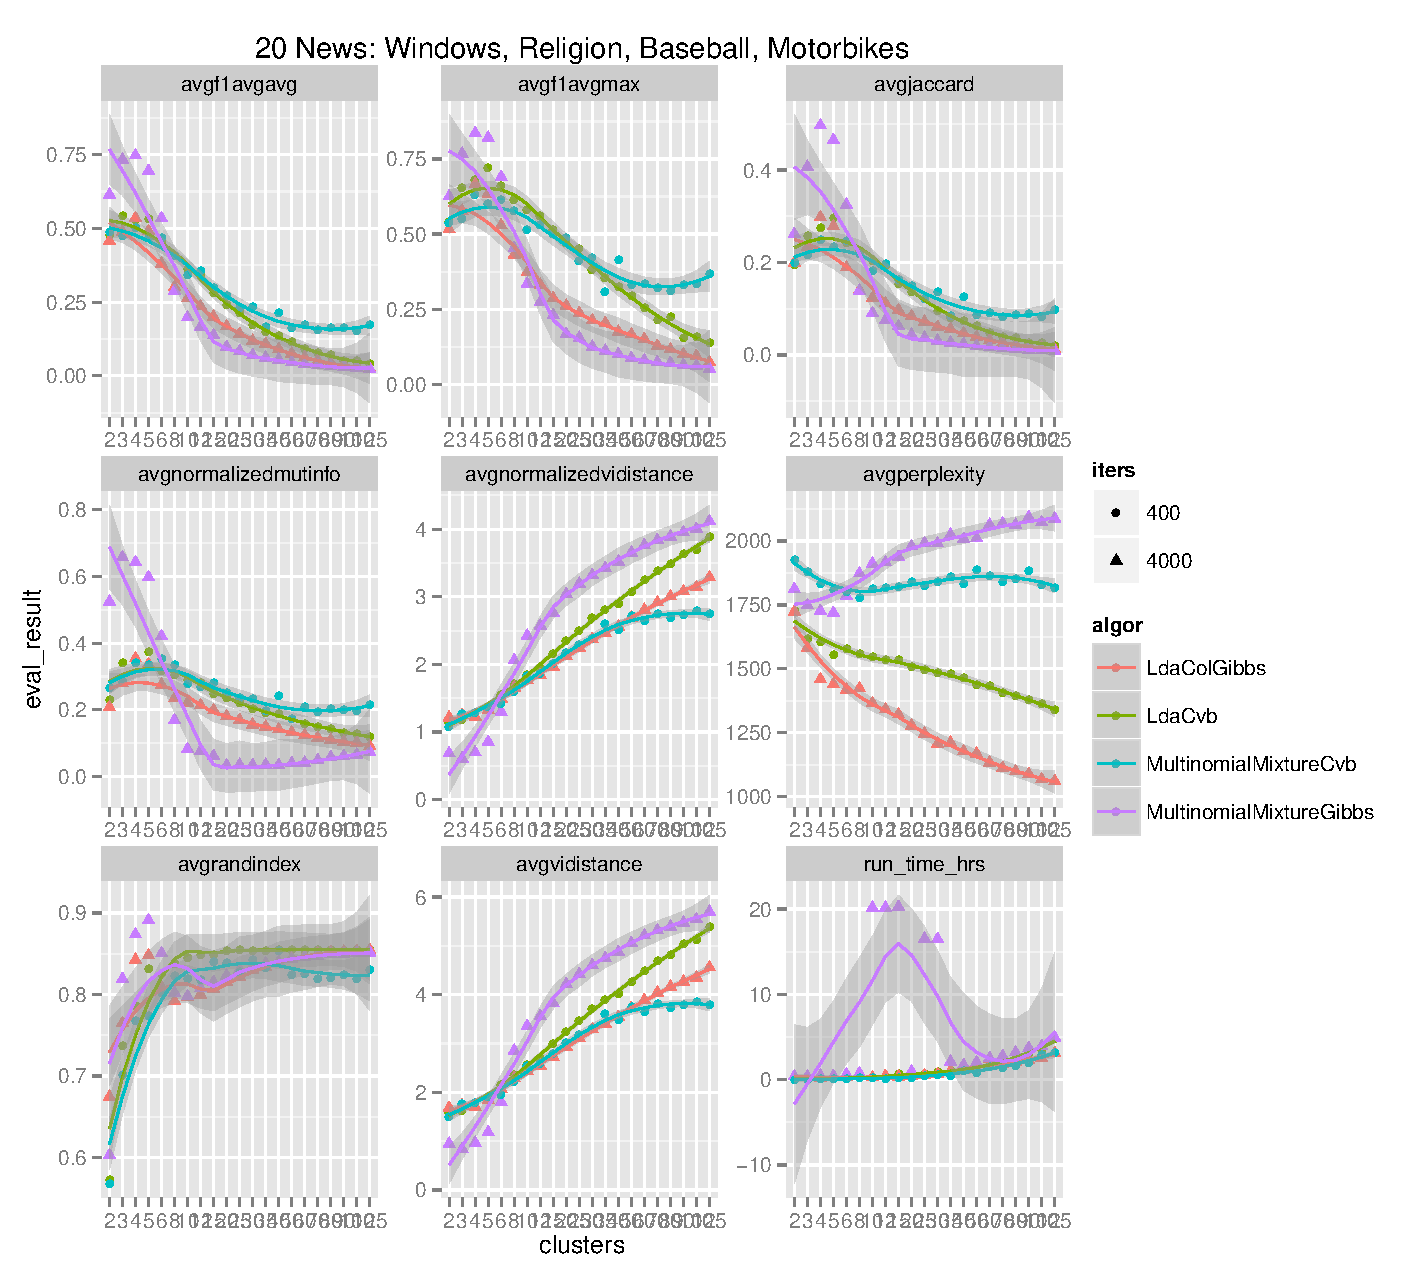
\includegraphics[width=0.9\textwidth]{../Chap3a/plots/20news-2013-03-25.pdf}
  \caption{Results using different accuracy metrics for a mixture of multinomials and LDA on a subset of the 20-news dataset. Trendlines and shading are from a LOESS fit to the points. A variation of the soft F1 measure described in the text is shown where we average over label-specific F1 scores instead of taking the maximum. Held-out likelihood was evaluating using the document-completion metric with inferred topics.}
  \label{fig:eval-metrics-shootout}
\end{figure}


A different approach to comes from the intuition that given two equivalent labelings, one would expect label pairs $z=k$ and $t=l$ to co-occur, and so expect that $p(z,t) \neq p(z)p(t)$, which opens the door to a number of information theoretic measures such as normalised mutual information (NMI) and the Variation of Information (VI) distance..

\newcommand{\TopDist}{\Theta}
\newcommand{\LabDist}{\mathbb{C}}
\newcommand{\NMI}{\text{NMI}}

Given a corpus-wide distribution over topics $\TopDist$ and a corpus wide distribution over labels $\LabDist$ the NMI is defined as a function of the mutual information $\mut{\TopDist}{\LabDist}$

\begin{align}
\NMI & = \frac{\mut{\TopDist}{\LabDist}}{1/2(\ent{\TopDist} + \ent{\LabDist})} &
\mut{\TopDist}{\LabDist} & = \sum_k \sum_l p(\theta_{\cdot k}, t_{\cdot l}) \ln \frac{p(\theta_{\cdot k}, t_{\cdot l})}{p(\theta_{\cdot k})p(t_{\cdot l})}
\end{align}
and the entropies are defined as
\begin{align}
\ent{\TopDist} & = - \sum_k p(\theta_{\cdot k}) \ln (\theta_{\cdot k}) &
\ent{\LabDist} & = - \sum_l p(t_{\cdot l}) \ln p(t_{\cdot l})
\end{align}

In the case of LDA these distributions would be defined as
\begin{align}
p(\theta_{\cdot k}) & =  \frac{1}{D} \sum_d \theta_{dk} ,&
p(t_{\cdot l}) &= \frac{1}{D'} \sum_d t_{dl} ,& 
p(\theta_{\cdot k}, t_{\cdot l}) & = \frac{1}{D'} \sum_d \theta_{dk} t_{dl}
\end{align}
where again $D' = \sum_d \sum_l t_{dl}$ is the total number of label instances, such that $D' \geq D$


The VI distance\cite{Meila2003} is another information-theoretic measure defined over a topic distribution $\TopDist$ and labelling distribution $\LabDist$ as:
\begin{equation}
\dvi{\TopDist}{\LabDist} = \ent{\LabDist} + \ent{\TopDist} - 2 \mut{\LabDist}{\TopDist}.
\end{equation}

$\dvi{\TopDist}{\LabDist}$ is a true metric: it is always non-negative, becomes zero if and only if $\LabDist = \TopDist$, is symmetric, and observes the triangle inequality, $\dvi{X}{Z} + \dvi{Z}{Y} \geq \dvi{X}{Y}$. However the range over which VI distance scores will take is dataset-dependant, and so to compare scores across datasets one can use the \emph{normalized VI distance}\cite{Reichart2009} which is defined as. 

\begin{align}
\text{NVI}\left[ \TopDist, \LabDist \right] = \left\{ \begin{array}{lr}
     \frac{1}{\ent{\TopDist}}\dvi{\TopDist}{\LabDist} & \ent{\TopDist} \neq 0 \\
     \ent{\LabDist} & \text{otherwise}
 \end{array}\right.
\end{align}


The VI distance has been used to compare topics inferred by LDA with manual labelling of over 20,000 news-stores in \cite{HeinrichEtAl2005}. 


A well-known metric from the field of clustering is the rand Rand Index, which determines how similar are two ways of partitioning data. It counts fours classes of document-pairs: (a) those which have the same cluster and have the same label; (b) those which have different clusters but share the same label; (c) those which have the same cluster but have different labels; and (d) those which which are not in the same cluster and have different labels.

Given these definitions the index is then $\text{RI} = \frac{a + d}{a + b + c + d}$. This is broadly similar to the idea of accuracy traditionally defined as being $\frac{TP + TN}{TP + FN + FP + TN}$

For the kind of soft-clustering featured in LDA, one would define these counts as
\begin{equation}
\begin{aligned}
a & = \sum_k \sum_{d, {p>d}} \theta_{dk} \theta_{pk} \sum_l t_{dl}t_{pl} & \quad
b & = \sum_k \sum_{d, {p>d}} \theta_{dk} (1 -\theta_{pk}) \sum_l t_{dl}t_{pl}\\
c & = \sum_k \sum_{d, {p>d}} \theta_{dk} \theta_{pk} \sum_{l,m \neq l} t_{dl}t_{ml} & \quad
d & = \sum_k \sum_{d, {p>d}} \theta_{dk} (1- \theta_{pk}) \sum_{l,m \neq l} t_{dl}t_{ml}
\end{aligned}
\end{equation}

Plots of all these metrics, for different topic counts, are given in figure \ref{fig:eval-metrics-shootout} for documents taken from four very different newsgroups from the overall 20-newsgroups dataset.



\bibliographystyle{plain}
\bibliography{/Users/bryanfeeney/Documents/library.bib}

\end{document}

